\documentclass[output=paper]{LSP/langsci}
\author{Bryan James Gordon}
\title{Information-structural variations in Siouan languages}
\abstract{Most previous information-structural analysis on Siouan languages has been fragmentary and based on incommensurable definitions and frameworks. A corpus study drawing on transcribed and recorded utterances from languages in all major branches of Siouan represents a first step towards generalizable and practical knowledge of the morphosyntactic and intonational indices of information-structural categories in Siouan languages. This study focuses on variations previously noted in the literature -- intonational marking and demarking, postverbal arguments, reduction of referring expressions, OSV word order and switch-topic markers. KEYWORDS: [information structure, intonation, postverbal arguments, word order, switch-topic markers, link, recoverability, topic, focus]}
\maketitle

\begin{document}

\section{Introduction}

<<<<<<< HEAD
	The formal linguistic record offers excellent, comprehensive documentation of morphological, syntactic and phonological structures in Siouan languages. The documentary record of those forms’ functions and meanings, however, is hit-and-miss -- fragmented, uncomprehensive, and characterized by individual linguists’ often incommensurable functional analytical frameworks. Most of us documentary linguists, in fact, have been trained to seek out, describe and privilege descriptions of context-free levels of semantic meaning, and our work has less to say about the meanings that emerge in and create our linguistic and social contexts, which may well be the most important types of meanings to community-based language-reclamation projects who try to adapt and use our work. The work I present here, while not free of its own analytical framework, attempts to rectify this situation by providing a comprehensive albeit partial description of one area of functional variation in form -- information structure -- based on a largely qualitative corpus study sampling data from nine Siouan languages.
	
	Most, if not all, previous descriptions of Siouan grammars have had something to say about information structure. \citet{Rudin1998}, \citet{Koontz2003} and \citet{Eschenberg2005} provide grammar/discourse analyses of specific features of Umoⁿhoⁿ Iye (Omaha). Graczyk (1991: 242-60) and de \citet{Reuse1994} describe the functions of noun incorporation in Apsaalooke (Crow) and Lakȟol’iapi (Lakota), respectively. Rood offers analyses of presupposition (1977) and variation between definite articles (1985), also in Lakȟol’iapi. \citet{Kaufman2008} offers some information-structural analysis of Taneks (Biloxi).\todo{there was a null byte here. Is the encoding OK?} \citet{Wolvengrey1990} describes a switch-topic marker (a “focus” marker in his terms) in Rų’eta (Mandan). Issues of “oldness”, “emphasis”, “topic” and “focus” surface in various formal grammars including Cumberland’s (2005) Nakʰon’i’a (Assiniboine) and Boyle’s (2007) Hidatsa grammar. Ingham’s work (2003) is a notably comprehensive discourse-analytical approach to information-structural variations in La\-kȟol\-’ia\-pi. These works, however, generally focus on a single phenomenon, and do not all situate themselves as relevant to a more general field of information-structurally meaningful variation. 
	
	Here I adopt a toolkit which allows us to unify, enrich and extend previous findings under a common descriptive metalanguage. My hope is not so much to argue for or against previous analysts’ theoretical or methodological goals (or my own, despite the fact that I necessarily highlight my own), but to make possible a more coherent and useful conversation about Siouan information-structural variations for a variety of audiences, including but not limited to theoretical linguists and community-based language-reclamation programs.

\section{Method}

For this study I coded interlinear text from nine languages, and audio data from four, a corpus comprising the majority of text and audio available to me at time of study in 2009. These languages span the four branches of the Siouan language family, including all three subbranches of the large Mississippi Valley Siouan subfamily: Rų’eta (Mandan\footnote{I use autonyms where available for language names, providing the English colonial name in parentheses only on first mention. It should not be assumed that the autonyms have the same reference as English colonial names. “Mandan”, for example, refers to a group of related varieties of which Rų’eta is only one.}); Taneksą (Biloxi - Ohio Valley Siouan); Hidatsa and Apsaalooke (Crow - Missouri Valley Siouan); and the Mississippi Valley Siouan languages Nakʰon’i’a (Assiniboine), Lakȟol’iapi (Lakota), Umoⁿhoⁿ Iye and Paⁿka Iye (Omaha and Ponca), Hoocąk (Winnebago), and Baxoje Ich\^{}e and Jiwere Ich\^{}e (Ioway and Otoe). Of these I was able to access audio data in Hidatsa, Umoⁿhoⁿ Iye, Baxoje Ich\^{}e and Hocąk. My sample, although representative of genetic diversity within the Siouan family, is not balanced across considerations of genre, time period or other sociolinguistic factors. These sources and the speakers who produced them are listed, with an utterance or page count, under the “Primary Resources” section of the bibliography. I coded each primary resource for formal variation (intonational, segmental and morphosyntactic criteria summarized in \sectref{intonationcoding}--\ref{variantselection}) and information-structural function (criteria summarized in \sectref{informationcoding}). Some of these resources I coded in their entirety; in others (e.g. Dorsey, 1890) I simply sampled a few works, attempting to capture multiple genres. I also drew many examples for this paper from secondary resources, and they are cited as such when they occur.

\subsection{Information-structural coding procedure}\label{informationcoding}

The following is a condensed version of my coding criteria. My criteria are drawn with some modification from the Givenness Hierarchy (Gundel et al. 1993) and Ward \& Birner’s (2001) framework, with attention towards commensurability with other frameworks. Because commensurability is one of my objectives, I do not use the terms given, old, topic or focus without specifying modifiers and definitions. I am the sole coder, so I have no intercoder reliability measure for these criteria, but it may be noted that I was applying Gundel’s criteria in the Minnesota Cognitive Status Research Group\footnote{The Minnesota Cognitive Status Research Group was funded by a National Science Foundation grant, \textit{A cross-linguistic study of reference and cognitive status} (BCS0519890, PI Jeanette Gundel).} at the time this study was conceived, and that we achieved 85\% intercoder reliability. All errors and misapplications are my own.

\ea\label{codingcriteria}
\ea{Code a form as a \textsc{link} if its referent stands in a poset relation with a salient or inferrable alternative. See Ward \& Birner (2001: 121) for examples, and cf. the categories of \textsc{contrast} and \textsc{restriction} in \citet{Erteschik-Shir2007}. Forms coded as links are \underline{underlined}.}
\ex{Code a form as \textsc{recoverable} if its referent is an \textsc{attention-central} entity or an \textsc{inferrable} predicate. These categories are operationalized as in Gundel et al. (1993, 2010), but I replace Gundel’s term \textsc{in focus} with \textsc{attention-central} to avoid confusion with relational focus. A referent is attention-central if its utterer can assume that her audience is consciously attending to it (cf. \textsc{continuing topic} in Erteschik-Shir, 2007, and \textsc{highly accessible} in Ariel, 1990). A referent is inferrable if the discourse model at time of reference gives ample and recoverable evidence for its validity (if a predicate) or existence (if an entity). Such evidence may be logical, narrative, stereotypic or based on general cultural knowledge. Forms coded as recoverable are \textit{italicized}.}
\ex{Code a form as a \textsc{relational topic} or \textsc{relational focus} if its referent stands in a directed relation (i.e., a relationship of semantic scope like quantification, or pragmatic/framing scope in the sense of Goffman 1974, e.g. stage topics, scene-modifiers, activating topics, extragrammatical mentions, unactivated definites, deixis, “aboutness” and “predication-of”). Relational topics are forms whose referents take scope, and relational foci are forms whose referents are under scope. Forms coded as relational topics are followed by a right angle bracket >, while those coded as relational foci are followed by a left angle bracket <.}\z
=======
	The formal linguistic record offers excellent, comprehensive documentation of morphological, syntactic and phonological structures in Siouan languages. The documentary record of those forms??? functions and meanings, however, is hit-and-miss -- fragmented, uncomprehensive, and characterized by individual linguists??? often incommensurable functional analytical frameworks. Most of us documentary linguists, in fact, have been trained to seek out, describe and privilege descriptions of context-free levels of semantic meaning, and our work has less to say about the meanings that emerge in and create our linguistic and social contexts, which may well be the most important types of meanings to community-based language-reclamation projects who try to adapt and use our work. The work I present here, while not free of its own analytical framework, attempts to rectify this situation by providing a comprehensive albeit partial description of one area of functional variation in form -- information structure -- based on a largely qualitative corpus study sampling data from nine Siouan languages.
	
	Most, if not all, previous descriptions of Siouan grammars have had something to say about information structure. Rudin (1998), Koontz (2003) and Eschenberg (2005) provide grammar/discourse analyses of specific features of Umo???ho??? Iye (Omaha). Graczyk (1991: 242-60) and de Reuse (1994) describe the functions of noun incorporation in Apsaalooke (Crow) and Lak??ol???iapi (Lakota), respectively. Rood offers analyses of presupposition (1977) and variation between definite articles (1985), also in Lak??ol???iapi. Kaufman (2008) offers some information-structural analysis of Taneks? ?(Biloxi). Wolvengrey (1990) describes a switch-topic marker (a ???focus??? marker in his terms) in R?????eta (Mandan). Issues of ???oldness???, ???emphasis???, ???topic??? and ???focus??? surface in various formal grammars including Cumberland???s (2005) Nak??on???i???a (Assiniboine) and Boyle???s (2007) Hidatsa grammar. Ingham???s work (2003) is a notably comprehensive discourse-analytical approach to information-structural variations in La\-k??ol\-???ia\-pi. These works, however, generally focus on a single phenomenon, and do not all situate themselves as relevant to a more general field of information-structurally meaningful variation. 
	
	Here I adopt a toolkit which allows us to unify, enrich and extend previous findings under a common descriptive metalanguage. My hope is not so much to argue for or against previous analysts??? theoretical or methodological goals (or my own, despite the fact that I necessarily highlight my own), but to make possible a more coherent and useful conversation about Siouan information-structural variations for a variety of audiences, including but not limited to theoretical linguists and community-based language-reclamation programs.

\section{Method}

For this study I coded interlinear text from nine languages, and audio data from four, a corpus comprising the majority of text and audio available to me at time of study in 2009. These languages span the four branches of the Siouan language family, including all three subbranches of the large Mississippi Valley Siouan subfamily: R?????eta (Mandan\footnote{I use autonyms where available for language names, providing the English colonial name in parentheses only on first mention. It should not be assumed that the autonyms have the same reference as English colonial names. ???Mandan???, for example, refers to a group of related varieties of which R?????eta is only one.}); Taneks?? (Biloxi - Ohio Valley Siouan); Hidatsa and Apsaalooke (Crow - Missouri Valley Siouan); and the Mississippi Valley Siouan languages Nak??on???i???a (Assiniboine), Lak??ol???iapi (Lakota), Umo???ho??? Iye and Pa???ka Iye (Omaha and Ponca), Hooc??k (Winnebago), and Baxoje Ich\^{}e and Jiwere Ich\^{}e (Ioway and Otoe). Of these I was able to access audio data in Hidatsa, Umo???ho??? Iye, Baxoje Ich\^{}e and Hoc??k. My sample, although representative of genetic diversity within the Siouan family, is not balanced across considerations of genre, time period or other sociolinguistic factors. These sources and the speakers who produced them are listed, with an utterance or page count, under the ???Primary Resources??? section of the bibliography. I coded each primary resource for formal variation (intonational, segmental and morphosyntactic criteria summarized in ??\ref{intonationcoding}--\ref{variantselection}) and information-structural function (criteria summarized in ??\ref{informationcoding}). Some of these resources I coded in their entirety; in others (e.g. Dorsey, 1890) I simply sampled a few works, attempting to capture multiple genres. I also drew many examples for this paper from secondary resources, and they are cited as such when they occur.

\subsection{Information-structural coding procedure}\label{informationcoding}

The following is a condensed version of my coding criteria. My criteria are drawn with some modification from the Givenness Hierarchy (Gundel et al. 1993) and Ward \& Birner???s (2001) framework, with attention towards commensurability with other frameworks. Because commensurability is one of my objectives, I do not use the terms given, old, topic or focus without specifying modifiers and definitions. I am the sole coder, so I have no intercoder reliability measure for these criteria, but it may be noted that I was applying Gundel???s criteria in the Minnesota Cognitive Status Research Group\footnote{The Minnesota Cognitive Status Research Group was funded by a National Science Foundation grant, \textit{A cross-linguistic study of reference and cognitive status} (BCS0519890, PI Jeanette Gundel).} at the time this study was conceived, and that we achieved 85\% intercoder reliability. All errors and misapplications are my own.

\ea\label{codingcriteria}
\ea{Code a form as a \textsc{link} if its referent stands in a poset relation with a salient or inferrable alternative. See Ward \& Birner (2001: 121) for examples, and cf. the categories of \textsc{contrast} and \textsc{restriction} in Erteschik-Shir (2007). Forms coded as links are \underline{underlined}.}
\ex{Code a form as \textsc{recoverable} if its referent is an \textsc{attention-central} entity or an \textsc{inferrable} predicate. These categories are operationalized as in Gundel et al. (1993, 2010), but I replace Gundel???s term \textsc{in focus} with \textsc{attention-central} to avoid confusion with relational focus. A referent is attention-central if its utterer can assume that her audience is consciously attending to it (cf. \textsc{continuing topic} in Erteschik-Shir, 2007, and \textsc{highly accessible} in Ariel, 1990). A referent is inferrable if the discourse model at time of reference gives ample and recoverable evidence for its validity (if a predicate) or existence (if an entity). Such evidence may be logical, narrative, stereotypic or based on general cultural knowledge. Forms coded as recoverable are \textit{italicized}.}
\ex{Code a form as a \textsc{relational topic} or \textsc{relational focus} if its referent stands in a directed relation (i.e., a relationship of semantic scope like quantification, or pragmatic/framing scope in the sense of Goffman 1974, e.g. stage topics, scene-modifiers, activating topics, extragrammatical mentions, unactivated definites, deixis, ???aboutness??? and ???predication-of???). Relational topics are forms whose referents take scope, and relational foci are forms whose referents are under scope. Forms coded as relational topics are followed by a right angle bracket >, while those coded as relational foci are followed by a left angle bracket <.}\z
>>>>>>> 374260aa11eac38304f850062805c954c530b1e7
\z

Example \ref{codingsummary} diagrammatically represents the coding marks as they are presented in all examples taken from primary sources:

\ea\label{codingsummary}{\underline{link}\hspaceThis{mm} \textit{recoverable}\hspaceThis{mm} relational topic >\hspaceThis{mm} relational focus <}\z

\subsection{Intonation-structural coding procedure}\label{intonationcoding}

<<<<<<< HEAD
Armik \citet{Mirzayan2011} has developed a ToBI coding protocol (cf. Pierrehumbert 1980; Beckman \& Pierrehumbert 1986; and Pierrehumbert \& Hirschberg 1990) for Lakȟol’iapi, but at the time of this study no such protocol was available, so I developed one myself. This section principally includes the basic description and justification of the protocol I developed; precise coding criteria have been omitted for length considerations and are available on request. 

The four sampled languages display the standard array of prosodic phrase levels: the \textsc{accent phrase} (AccP), the \textsc{intermediate phrase} (IntP) and the \textsc{intonational phrase} (IP). Accent phrases in all four languages maximally consist of a low-high-low contour in which either the high point or the high-low fall is accorded greatest prosodic prominence. Such contours are represented in ToBI notation as LH*L, and all four languages have them, although the first L tone in particular is often absent. Intermediate phrases in all four languages consist of one or more accent phrases followed by a phrase accent, either !H or L; and intonational phrases in all four languages consist of one or more intermediate phrases followed by a boundary tone, either !H\% or L\%. The exclamation point before H phrase accents and boundary tones indicates downstep: I found no evidence of upstepped H phrase accents or boundary tones in any of the four languages. 

My protocol was designed to cover four languages (Umoⁿhoⁿ Iye, Hocąk, Baxoje Ich\^{}e and Hidatsa) rather than one, and so is shallower and less detailed than Mirzayan’s. The simple apparatus sketched here is designed to capture high-level intonational variations across Siouan languages, and should not be taken as evidence that Siouan intonational structures are simple. Besides Mirzayan (ib.) see \citet{Larson2009} on Umoⁿhoⁿ Iye for richer descriptions of intonational variation in particular Siouan languages. 

\subsection{Selection of formal variants of interest}\label{variantselection}

In information structure and intonational structure I have begun with high-level, a priori coding categories and attempted to apply them to the entire corpus. In deciding which formal (morphosyntactic and segmental as well as intonational) variations to correlate to information structure, however, I have made no such attempt. Instead, I have specifically looked at some of the formal variations in previous descriptions of Siouan languages: postverbal arguments (\sectref{postverbalarguments}); degrees of reduction of noun phrases or referring expressions, from zero reference to “determiner drop” and noun incorporation (\sectref{nominalreduction}); OSV word order (\sectref{osv}); switch-topic markers (\sectref{switchtopic}); and intonational processes of “marking” and “demarking” which surfaced during my ToBI coding (\sectref{intonationalbounding} and \sectref{deaccenting}, respectively).
=======
Armik Mirzayan (2011) has developed a ToBI coding protocol (cf. Pierrehumbert 1980; Beckman \& Pierrehumbert 1986; and Pierrehumbert \& Hirschberg 1990) for Lak??ol???iapi, but at the time of this study no such protocol was available, so I developed one myself. This section principally includes the basic description and justification of the protocol I developed; precise coding criteria have been omitted for length considerations and are available on request. 

The four sampled languages display the standard array of prosodic phrase levels: the \textsc{accent phrase} (AccP), the \textsc{intermediate phrase} (IntP) and the \textsc{intonational phrase} (IP). Accent phrases in all four languages maximally consist of a low-high-low contour in which either the high point or the high-low fall is accorded greatest prosodic prominence. Such contours are represented in ToBI notation as LH*L, and all four languages have them, although the first L tone in particular is often absent. Intermediate phrases in all four languages consist of one or more accent phrases followed by a phrase accent, either !H or L; and intonational phrases in all four languages consist of one or more intermediate phrases followed by a boundary tone, either !H\% or L\%. The exclamation point before H phrase accents and boundary tones indicates downstep: I found no evidence of upstepped H phrase accents or boundary tones in any of the four languages. 

My protocol was designed to cover four languages (Umo???ho??? Iye, Hoc??k, Baxoje Ich\^{}e and Hidatsa) rather than one, and so is shallower and less detailed than Mirzayan???s. The simple apparatus sketched here is designed to capture high-level intonational variations across Siouan languages, and should not be taken as evidence that Siouan intonational structures are simple. Besides Mirzayan (ib.) see Larson (2009) on Umo???ho??? Iye for richer descriptions of intonational variation in particular Siouan languages. 

\subsection{Selection of formal variants of interest}\label{variantselection}

In information structure and intonational structure I have begun with high-level, a priori coding categories and attempted to apply them to the entire corpus. In deciding which formal (morphosyntactic and segmental as well as intonational) variations to correlate to information structure, however, I have made no such attempt. Instead, I have specifically looked at some of the formal variations in previous descriptions of Siouan languages: postverbal arguments (??\ref{postverbalarguments}); degrees of reduction of noun phrases or referring expressions, from zero reference to ???determiner drop??? and noun incorporation (??\ref{nominalreduction}); OSV word order (??\ref{osv}); switch-topic markers (??\ref{switchtopic}); and intonational processes of ???marking??? and ???demarking??? which surfaced during my ToBI coding (??\ref{intonationalbounding} and ??\ref{deaccenting}, respectively).
>>>>>>> 374260aa11eac38304f850062805c954c530b1e7

\section{Findings}\label{findings}

\subsection{Deaccenting}\label{deaccenting}

<<<<<<< HEAD
	I use the term \textsc{deaccenting} to describe intonational variations in which a given word or string of words may be realized either with or without the H* pitch-accent head of an AccP. The variant without the pitch accent is the \textsc{deaccented} variant. This term implies that the accented variant is canonical. Bolinger (1986: 100) makes this explicit: “[A] neutral sentence accents all content words, … and a non-neutral or marked sentence would be one in which one or more words have been deaccented.”
	
Every audio resource I coded has examples of deaccenting, and all examples of deaccenting signal a recoverable referent. In example \ref{wolfedeaccenting}, Umoⁿhoⁿ Iye speaker Clifford Wolfe, Sr., deaccents the strings \textit{kʰi égithe “and so it happened that”} and \textit{ahíi “arrived there”}. Both are absorbed into the LH*L contour of the AccP headed by \textit{weáhidexti “truly far”}:

\ea\label{wolfedeaccenting}
Shkóⁿ-tʰe wasékoⁿ, kʰi égithe weáhidexti ahí.\footnotemark

\glll 	\emph{shkóⁿ-tʰe >}	\emph{wasékoⁿ <}		kʰi 		égithe 		\emph{weáhidexti}		{ahí <}\\
	{\ob L H* L\cb}		{\ob L !H* L\cb\hspaceThis{ }L}		{\ob L}	{}			{H* L}				{\hspaceThis{ahí}\cb\hspaceThis{ }L L\%}\\
=======
	I use the term \textsc{deaccenting} to describe intonational variations in which a given word or string of words may be realized either with or without the H* pitch-accent head of an AccP. The variant without the pitch accent is the \textsc{deaccented} variant. This term implies that the accented variant is canonical. Bolinger (1986: 100) makes this explicit: ???[A] neutral sentence accents all content words, ??? and a non-neutral or marked sentence would be one in which one or more words have been deaccented.???
	
Every audio resource I coded has examples of deaccenting, and all examples of deaccenting signal a recoverable referent. In example \ref{wolfedeaccenting}, Umo???ho??? Iye speaker Clifford Wolfe, Sr., deaccents the strings \textit{k??i ??githe ???and so it happened that???} and \textit{ah??i ???arrived there???}. Both are absorbed into the LH*L contour of the AccP headed by \textit{we??hidexti ???truly far???}:

\ea\label{wolfedeaccenting}
Shk?????-t??e was??ko???, k??i ??githe we??hidexti ah??.\footnotemark

\glll 	\emph{shk?????-t??e >}	\emph{was??ko??? <}		k??i 		??githe 		\emph{we??hidexti}		{ah?? <}\\
	{\ob L H* L\cb}		{\ob L !H* L\cb\hspaceThis{ }L}		{\ob L}	{}			{H* L}				{\hspaceThis{ah??}\cb\hspaceThis{ }L L\%}\\
>>>>>>> 374260aa11eac38304f850062805c954c530b1e7
	movement-the 		fast 				and 		it.happened.that 	ahead.really	 		arrive.there.\textsc{prox}\\
\footnotetext{Rudin field tapes}
\glt She was moving fast, so it happened that she got pretty far ahead.
\z

<<<<<<< HEAD
In example \ref{wolfedeaccenting} and in other audio examples, I provide a ToBI line under the information-structural coding and above the gloss line. Here, AccP’s are represented by square brackets. IntP’s are recognisable by their pitch accents outside square brackets, and the IP by its boundary tone. 
=======
In example \ref{wolfedeaccenting} and in other audio examples, I provide a ToBI line under the information-structural coding and above the gloss line. Here, AccP???s are represented by square brackets. IntP???s are recognisable by their pitch accents outside square brackets, and the IP by its boundary tone. 
>>>>>>> 374260aa11eac38304f850062805c954c530b1e7

For this example, I also provide a praat screenshot, but omit it from subsequent examples due to space considerations. In the screenshot, the blue line is the pitch contour in Hz, and the green line the intensity contour in dB.\footnote{It should further be noted that the blue line, being a computed estimate of pitch, is not sufficient evidence for any ToBI coding criterion, but must be accompanied by impressionistic auditing.} The ToBI line in my praat annotations is simplified relative to the ToBI line in the examples presented in this paper. Glosses in the praat annotations my provided at the IntP level, which is a technique I use to simulate the intermediate-level prosodic chunking present in the audio.

\begin{figure}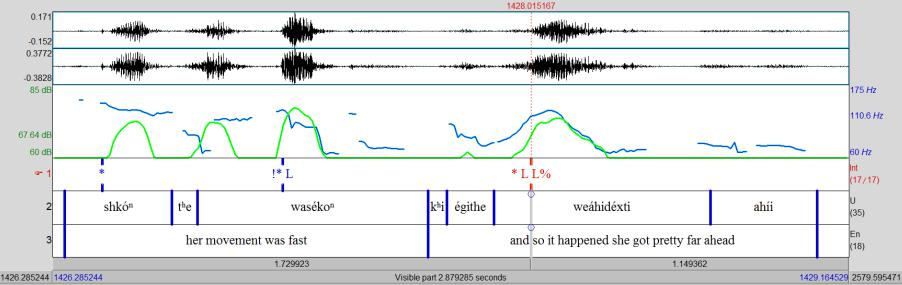
\includegraphics[width=12cm]{figures/Gordon1}\caption{praat screenshot corresponding to example \ref{wolfedeaccenting}}\label{wolfedeaccentingscreenshot}\end{figure}

<<<<<<< HEAD
In example \ref{wolfedeaccenting}, two sections have been deaccented and absorbed into the L tones that bound an adjacent H* phrase accent. Both have been coded as recoverable: \textit{kʰi égithe} because it is a frequent discourse marker that is likely always recoverable in narrative. The predicate \textit{ahíi} is inferrable given immediately preceding references to motion, speed and distance.

We may distinguish between “true” deaccenting, as in example \ref{wolfedeaccenting}, where the deaccented part of the pitch contour is either flat or very slowly declining, and “weak” deaccenting, as in example \ref{wolfeweakdeaccenting}, where Mr. Wolfe uses a compressed version of the LH*L contour. We are looking at \textit{níkshiⁿga}, whose ToBI line is annotated with (LM*L). This is because the pitch range of this contour is compressed within a range smaller than the pitch range of the L tone in the adjacent AccP, so that it is realized as something more like (LM*L) than a full [LH*L] AccP.

\ea\label{wolfeweakdeaccenting}
Hiⁿbéazhi-tʰe égithe, táxti sí-tʰe, thiwágazui níkshiⁿga.\footnotemark
\glll	\emph{\underline{hiⁿbé-ázhi-tʰe}}	{\underline{égithe} >}				\emph{\underline{táxti}}		\emph{\underline{sí-tʰe} <}		\emph{thiwágazui}	\emph{níkshiⁿga}\\
	{\ob L H* L}					{\hspaceThis{égithe}\cb\hspaceThis{ }!H}	{\ob L H* L\cb}			{\ob L !H* L\cb}				{\ob L H* L}			{\op \textsc{l m* l}\cp\cb\hspaceThis{ }L L\%}\\
=======
In example \ref{wolfedeaccenting}, two sections have been deaccented and absorbed into the L tones that bound an adjacent H* phrase accent. Both have been coded as recoverable: \textit{k??i ??githe} because it is a frequent discourse marker that is likely always recoverable in narrative. The predicate \textit{ah??i} is inferrable given immediately preceding references to motion, speed and distance.

We may distinguish between ???true??? deaccenting, as in example \ref{wolfedeaccenting}, where the deaccented part of the pitch contour is either flat or very slowly declining, and ???weak??? deaccenting, as in example \ref{wolfeweakdeaccenting}, where Mr. Wolfe uses a compressed version of the LH*L contour. We are looking at \textit{n??kshi???ga}, whose ToBI line is annotated with (LM*L). This is because the pitch range of this contour is compressed within a range smaller than the pitch range of the L tone in the adjacent AccP, so that it is realized as something more like (LM*L) than a full [LH*L] AccP.

\ea\label{wolfeweakdeaccenting}
Hi???b??azhi-t??e ??githe, t??xti s??-t??e, thiw??gazui n??kshi???ga.\footnotemark
\glll	\emph{\underline{hi???b??-??zhi-t??e}}	{\underline{??githe} >}				\emph{\underline{t??xti}}		\emph{\underline{s??-t??e} <}		\emph{thiw??gazui}	\emph{n??kshi???ga}\\
	{\ob L H* L}					{\hspaceThis{??githe}\cb\hspaceThis{ }!H}	{\ob L H* L\cb}			{\ob L !H* L\cb}				{\ob L H* L}			{\op \textsc{l m* l}\cp\cb\hspaceThis{ }L L\%}\\
>>>>>>> 374260aa11eac38304f850062805c954c530b1e7
	moccasin-not-that				it-happened-that					deer					foot-that				notice-\textsc{prox}		person\\
\footnotetext{Rudin field tapes}
\glt	The man noticed that she was not wearing shoes, but rather had the feet of a deer.
\z

<<<<<<< HEAD
Mirzayan (2011: 121-3) presents similar compressed AccP’s in Lakȟol’iapi. This phenomenon may suggest a continuous process at work, in which the degree of accenting in AccP’s is continuously gradient. Such a process would challenge the usefulness of a discrete annotation system like ToBI for capturing deaccenting phenomena in Siouan languages. If this scale from “true” to “weak” deaccenting corresponds to variation in information-structural function, however, my coding criteria have not captured it. Instead, all types of deaccenting I have described signal recoverability of referents. This finding is entirely dependent on my methodology, however, and the area of gradient deaccenting and potential information-structural corollaries needs to be investigated further.
=======
Mirzayan (2011: 121-3) presents similar compressed AccP???s in Lak??ol???iapi. This phenomenon may suggest a continuous process at work, in which the degree of accenting in AccP???s is continuously gradient. Such a process would challenge the usefulness of a discrete annotation system like ToBI for capturing deaccenting phenomena in Siouan languages. If this scale from ???true??? to ???weak??? deaccenting corresponds to variation in information-structural function, however, my coding criteria have not captured it. Instead, all types of deaccenting I have described signal recoverability of referents. This finding is entirely dependent on my methodology, however, and the area of gradient deaccenting and potential information-structural corollaries needs to be investigated further.
>>>>>>> 374260aa11eac38304f850062805c954c530b1e7

In short, all the audio resources I coded display deaccented forms, and all such forms have recoverable referents.

\subsection{Postverbal arguments}\label{postverbalarguments}

<<<<<<< HEAD
Since all Siouan languages canonically position verbs after their arguments, the syntactic status of postverbal arguments is controversial. All Siouan languages at very least permit postsentential referring expressions to clarify one or more verbal arguments, but grammarians have varied in accepting postverbal arguments as elements of the same sentence (cf. Rudin 1998; Mithun 1999; Ingham 2003: 76; Cumberland 2005: 421; Boyle 2007: 292-3; Gordon 2008). My attention to deaccenting phenomena in this study may shed light on this question and enabling language workers to distinguish between those postverbal arguments which are clearly “outside” the sentences and those which are more likely “inside”.

Accented postverbal arguments (those which are pronounced with the [LH*L] contour of an AccP) typically have nonrecoverable referents. Instead, they clarify uncertain information, providing new information about both entities and predicates. (See Graczyk, 1991: 103, for a relevant discussion on Apsaalooke afterthought.) Accented postverbal arguments are usually separated from the verb not only by an AccP boundary but by a prosodic break (i.e. an IntP phrase accent or IP boundary tone). In example \ref{thigrepiraye}, Baxoje Ich\^{}e speaker ThigréPi concludes an IntP on \emph{ráye uⁿk\^{}úⁿñe\^{}suⁿ “they gave me a name”}, as seen in the L phrase accent, here evidenced by early and sustained low pitch. Then he adds another IntP in pronouncing the postverbal argument \emph{Baxóje ráye “a Baxoje name”}:

\ea\label{thigrepiraye}
Woxáñi migragáñi\^{}suⁿ, ráye, ráye uⁿk\^{}úⁿñe\^{}suⁿ, Baxóje ráye.\footnotemark\textsuperscript{,} \footnotemark\\
\glll	\emph{woxáñi} 	\emph{migragáñi\^{}suⁿ <}		\emph{ráye <}	ráye		\emph{uⁿk\^{}úⁿñe\^{}suⁿ <}	\emph{Baxóje <}		ráye\\
	{\ob L H* L}		{\hspaceThis{migragáñi\^{}s}L\cb}	{\ob L H* L L\cb}	{\ob L H* L}	{\hspaceThis{uⁿk\^{}úⁿñe}L\cb}	{\ob L !H* L} 		{L\cb\hspaceThis{ }L\%}\\
	cherished	me.their.named.now	name		name	me.give.\textsc{pl}.now	Ioway			name\\
\footnotetext{ThigréPi in \citet{GoodTracks2004}}
=======
Since all Siouan languages canonically position verbs after their arguments, the syntactic status of postverbal arguments is controversial. All Siouan languages at very least permit postsentential referring expressions to clarify one or more verbal arguments, but grammarians have varied in accepting postverbal arguments as elements of the same sentence (cf. Rudin 1998; Mithun 1999; Ingham 2003: 76; Cumberland 2005: 421; Boyle 2007: 292-3; Gordon 2008). My attention to deaccenting phenomena in this study may shed light on this question and enabling language workers to distinguish between those postverbal arguments which are clearly ???outside??? the sentences and those which are more likely ???inside???.

Accented postverbal arguments (those which are pronounced with the [LH*L] contour of an AccP) typically have nonrecoverable referents. Instead, they clarify uncertain information, providing new information about both entities and predicates. (See Graczyk, 1991: 103, for a relevant discussion on Apsaalooke afterthought.) Accented postverbal arguments are usually separated from the verb not only by an AccP boundary but by a prosodic break (i.e. an IntP phrase accent or IP boundary tone). In example \ref{thigrepiraye}, Baxoje Ich\^{}e speaker Thigr??Pi concludes an IntP on \emph{r??ye u???k\^{}?????n??e\^{}su??? ???they gave me a name???}, as seen in the L phrase accent, here evidenced by early and sustained low pitch. Then he adds another IntP in pronouncing the postverbal argument \emph{Bax??je r??ye ???a Baxoje name???}:

\ea\label{thigrepiraye}
Wox??n??i migrag??n??i\^{}su???, r??ye, r??ye u???k\^{}?????n??e\^{}su???, Bax??je r??ye.\footnotemark\textsuperscript{,} \footnotemark\\
\glll	\emph{wox????i} 	\emph{migrag????i\^{}su??? <}		\emph{r??ye <}	r??ye		\emph{u???k\^{}???????e\^{}su??? <}	\emph{Bax??je <}		r??ye\\
	{\ob L H* L}		{\hspaceThis{migrag????i\^{}s}L\cb}	{\ob L H* L L\cb}	{\ob L H* L}	{\hspaceThis{u???k\^{}???????e}L\cb}	{\ob L !H* L} 		{L\cb\hspaceThis{ }L\%}\\
	cherished	me.their.named.now	name		name	me.give.\textsc{pl}.now	Ioway			name\\
\footnotetext{Thigr??Pi in GoodTracks (2004)}
>>>>>>> 374260aa11eac38304f850062805c954c530b1e7
\footnotetext{Square brackets in the ToBI line here refer to IntP boundaries rather than AccP boundaries as previously.}
\glt	They named me as a cherished one, a name, they gave me a name, a Baxoje name.
\z

<<<<<<< HEAD
Deaccented postverbal arguments, in contrast -- like \emph{níkshiⁿga} in example \ref{wolfeweakdeaccenting} -- are not separated by prosodic breaks, and signal recoverable referents. Example \ref{wilkinsonpostverbal} is a useful model of the relationship between postverbal arguments and recoverability in general. Hidatsa speaker Helen Wilkinson says \emph{kúahe “this”} first in preverbal position when it is not recoverable, and then in postverbal position when in the second sentence (with the form \emph{kúac} it is recoverable:

\ea\label{wilkinsonpostverbal}
Kúahe aku-iháaraci. Maapúkšaruxpáaka wáahaapʰaak ráahaa’he ita-arukiwé’ kúac.\footnotemark\\
\gll	\emph{kúahe >}	\emph{aku-iháaraci <}	\emph{\underline{Maapúkšaruxpáaka}} 	\emph{\underline{wáahaapʰaak}} 	\emph{\underline{ráahaa’he}}			\emph{\underline{ita-arukiwé’} <}		kúac\\
=======
Deaccented postverbal arguments, in contrast -- like \emph{n??kshi???ga} in example \ref{wolfeweakdeaccenting} -- are not separated by prosodic breaks, and signal recoverable referents. Example \ref{wilkinsonpostverbal} is a useful model of the relationship between postverbal arguments and recoverability in general. Hidatsa speaker Helen Wilkinson says \emph{k??ahe ???this???} first in preverbal position when it is not recoverable, and then in postverbal position when in the second sentence (with the form \emph{k??ac} it is recoverable:

\ea\label{wilkinsonpostverbal}
K??ahe aku-ih??araci. Maap??k??aruxp??aka w??ahaap??aak r??ahaa???he ita-arukiw????? k??ac.\footnotemark\\
\gll	\emph{k??ahe >}	\emph{aku-ih??araci <}	\emph{\underline{Maap??k??aruxp??aka}} 	\emph{\underline{w??ahaap??aak}} 	\emph{\underline{r??ahaa???he}}			\emph{\underline{ita-arukiw?????} <}		k??ac\\
>>>>>>> 374260aa11eac38304f850062805c954c530b1e7
	Here.this 		different.sorta		Snake.People 					raid 						go.\textsc{caus}.that 				their.story.tell 					here.this\\
\footnotetext{Parks, Jones \& Hollow (1978: 18: 1)}
\glt	This is a different story [from the story of the Bird Woman]. This is the story of the Shoshone raid.
\z

<<<<<<< HEAD
There are some examples of multiple postverbal arguments. In example \ref{multiplepostverbal}, I present two. In example \ref{wilkinsonmultiplepostverbal}, Helen Wilkinson first gives us the recoverable postverbal argument \emph{maa-iháa’š “the enemy”} before then further specifying \emph{Waapúkšaruxpáaka’š “the Snake People”}. Although the two phrases share the same entity referent, the function of \emph{Waapúkšaruxpáaka’š} is to supply a predicate which is not inferrable at this point in the discourse model, so \emph{Waapúkšaruxpáaka’š} is coded nonrecoverable (one of the few unseparated by commas which I coded nonrecoverable). In example \ref{baxojemultiplepostverbal}, however, the telling of the Baxoje legend of Béñeiŋe recorded by Gordon \citet{Marsh1936} displays two postverbal arguments. Here the two are not coreferent, nor are they in the same argument relation to the verb, and they are both recoverable. 

\ea\label{multiplepostverbal}
\ea\label{wilkinsonmultiplepostverbal}
Hii šee awá ihtúutiru ú’šiak káawarec maa-iháa’š Waapúkšaruxpáaka’š.\footnotemark\\
\gll	hii 		\emph{šée} 		\emph{awá >}		\emph{ihtúutiru} 			\emph{ú’šiak} 		\emph{káawarec <}	maa-iháa’š 				\emph{Waapúkšaruxpáaka’š <}\\
=======
There are some examples of multiple postverbal arguments. In example \ref{multiplepostverbal}, I present two. In example \ref{wilkinsonmultiplepostverbal}, Helen Wilkinson first gives us the recoverable postverbal argument \emph{maa-ih??a????? ???the enemy???} before then further specifying \emph{Waap??k??aruxp??aka????? ???the Snake People???}. Although the two phrases share the same entity referent, the function of \emph{Waap??k??aruxp??aka?????} is to supply a predicate which is not inferrable at this point in the discourse model, so \emph{Waap??k??aruxp??aka?????} is coded nonrecoverable (one of the few unseparated by commas which I coded nonrecoverable). In example \ref{baxojemultiplepostverbal}, however, the telling of the Baxoje legend of B????ei??e recorded by Gordon Marsh (1936) displays two postverbal arguments. Here the two are not coreferent, nor are they in the same argument relation to the verb, and they are both recoverable. 

\ea\label{multiplepostverbal}
\ea\label{wilkinsonmultiplepostverbal}
Hii s??ee aw?? iht??utiru ?????s??iak k??awarec maa-ih??a???s?? Waap??k??aruxp??aka?????.\footnotemark\\
\gll	hii 		\emph{????e} 		\emph{aw?? >}		\emph{iht??utiru} 			\emph{???????iak} 		\emph{k??awarec <}	maa-ih??a????? 				\emph{Waap??k??aruxp??aka????? <}\\
>>>>>>> 374260aa11eac38304f850062805c954c530b1e7
	and 		that	 		ground 			hill.base.at	 			arrive.\textsc{ss} 		be.there.\textsc{pl.ne}	enemy.\textsc{pl.def}.the 		Snake.People.\textsc{pl.def}.the\\
\footnotetext{Parks, Jones \& Hollow (1978: 22: 26)}
\glt	And the enemy, the Shoshone, were on that ground, having gotten to the base of the hill.
\ex\label{baxojemultiplepostverbal}
<<<<<<< HEAD
Nahésge, igwáhuŋa súŋe Béñeiŋe.\footnotemark\\
\gll	\emph{nahésge >}	\emph{igwáhuŋa <}	súŋe 		Béñeiŋe\\
	be.if 			his.know 			horse 		Béñeiŋe\\
\footnotetext{\citet{Marsh1936}}
\glt	And so the horse\textsubscript{i} recognized his\textsubscript{i} [owner] Béñeiŋe.
\z\z

Without audio we can’t be sure whether the apparent double postverbal arguments are really all part of the same utterance, but it makes sense to speculate that, of the two, Ms. Wilkinson’s example is more likely to involve a major prosodic break than the Baxoje Ich\^{}e example.

In written transcripts for which no audio is available, I found the transcriber’s comma a somewhat useful index of prosody -- and recoverability. Many of the postverbal arguments I coded -- like Ms. Wilkinson’s in example \ref{wilkinsonpostverbal} -- were not separated by commas from preceding material. Although transcriber’s commas may somewhat reliably correlate with IntP or IP boundaries as annotated in ToBI, we cannot be too sure of how strong this correlation is. Still, nearly all of the postverbal arguments not separated by commas had recoverable referents. Presence of a comma, on the other hand, does not seem to reliably predict recoverability of the referent.

Not all languages (or speakers) are alike with respect to the frequency of postverbal arguments. I found many examples of postverbal reference to recoverable entities in Taneksą, Rų’eta, Hidatsa, and Umoⁿhoⁿ Iye and Paⁿka Iye texts, and very low rates in Hocąk and Apsaalooke texts -- but still nearly all of the postverbal arguments in the Hocąk and Apsaalooke texts I coded had recoverable referents. All the languages I looked at allow at least some use of postverbal arguments to refer to recoverable entities. In some languages, like Umoⁿhoⁿ Iye and Paⁿka Iye, this use may be (or have been) obligatory. In \citet{Gordon2008}, I sampled 51 continuing topics in Umoⁿhoⁿ Iye and Paⁿka Iye and found 42 of them were referred to postverbally. Of the 9 preverbal, most were within repeated collocations. This suggests that in some languages recoverable referents not only \emph{can} be referred to postverbally, but \emph{must} in most contexts.

To summarize, all the languages in this study make use of postverbal arguments, although they vary in frequency. Even without audio data to distinguish between deaccented and accented postverbal arguments, the strong tendency is observable for postverbal arguments to refer to recoverable entities. The index of the transcriber’s comma may serve as circumstantial evidence. Its absence indirectly indexes recoverability of postverbal referents while also directly, if weakly, indexing deaccenting. Forms with nonrecoverable referents are often found after commas, on the other hand. Where audio data is available, the case is clearer: deaccented postverbal arguments, like other deaccented material, have recoverable referents, and are intrasentential (part of the same sentence as the verb they follow) by intonational if not syntactic criteria.
=======
Nah??sge, igw??hu??a s????e B??n??ei??e.\footnotemark\\
\gll	\emph{nah??sge >}	\emph{igw??hu??a <}	s????e 		B????ei??e\\
	be.if 			his.know 			horse 		B????ei??e\\
\footnotetext{Marsh (1936)}
\glt	And so the horse\textsubscript{i} recognized his\textsubscript{i} [owner] B????ei??e.
\z\z

Without audio we can???t be sure whether the apparent double postverbal arguments are really all part of the same utterance, but it makes sense to speculate that, of the two, Ms. Wilkinson???s example is more likely to involve a major prosodic break than the Baxoje Ich\^{}e example.

In written transcripts for which no audio is available, I found the transcriber???s comma a somewhat useful index of prosody -- and recoverability. Many of the postverbal arguments I coded -- like Ms. Wilkinson???s in example \ref{wilkinsonpostverbal} -- were not separated by commas from preceding material. Although transcriber???s commas may somewhat reliably correlate with IntP or IP boundaries as annotated in ToBI, we cannot be too sure of how strong this correlation is. Still, nearly all of the postverbal arguments not separated by commas had recoverable referents. Presence of a comma, on the other hand, does not seem to reliably predict recoverability of the referent.

Not all languages (or speakers) are alike with respect to the frequency of postverbal arguments. I found many examples of postverbal reference to recoverable entities in Taneks??, R?????eta, Hidatsa, and Umo???ho??? Iye and Pa???ka Iye texts, and very low rates in Hoc??k and Apsaalooke texts -- but still nearly all of the postverbal arguments in the Hoc??k and Apsaalooke texts I coded had recoverable referents. All the languages I looked at allow at least some use of postverbal arguments to refer to recoverable entities. In some languages, like Umo???ho??? Iye and Pa???ka Iye, this use may be (or have been) obligatory. In Gordon (2008), I sampled 51 continuing topics in Umo???ho??? Iye and Pa???ka Iye and found 42 of them were referred to postverbally. Of the 9 preverbal, most were within repeated collocations. This suggests that in some languages recoverable referents not only \emph{can} be referred to postverbally, but \emph{must} in most contexts.

To summarize, all the languages in this study make use of postverbal arguments, although they vary in frequency. Even without audio data to distinguish between deaccented and accented postverbal arguments, the strong tendency is observable for postverbal arguments to refer to recoverable entities. The index of the transcriber???s comma may serve as circumstantial evidence. Its absence indirectly indexes recoverability of postverbal referents while also directly, if weakly, indexing deaccenting. Forms with nonrecoverable referents are often found after commas, on the other hand. Where audio data is available, the case is clearer: deaccented postverbal arguments, like other deaccented material, have recoverable referents, and are intrasentential (part of the same sentence as the verb they follow) by intonational if not syntactic criteria.
>>>>>>> 374260aa11eac38304f850062805c954c530b1e7

\subsection{Reduced nominal referring expressions}\label{nominalreduction}

\subsubsection{Determiner drop in languages with two indefinite articles}\label{droptwoindef}

<<<<<<< HEAD
Of the languages represented in this study, four -- Lakȟol’iapi, Nakʰon’i’a, Apsaalooke and Hocąk -- have two indefinite articles, one specific and one inspecific. The texts I coded in these four languages display determiner use in all nominal expressions which are specific (i.e. which refer to entities and not just to predicates or types) but nonrecoverable, allowing bare nominal expressions only for inspecific or recoverable referents\footnote{I do not consider generic reference in this study.}. In example \ref{stewartdrop} Apsaalooke speaker Francis Stewart refers twice to a specific quantity of water, but only the second reference is recoverable. This exemplifies how, among specific referents, recoverability makes the difference between determiner use and bare expressions:

\ea\label{stewartdrop}
Hinné wíliash kala iháatak huuk. Bilé xatáakelak.\footnotemark\\
\gll	\emph{\underline{hinné}} 	\emph{\underline{wilíash}} 		\emph{kala >} 	\emph{iháatak <}		\emph{huuk} 	bilé 		\emph{xatáakelak <}\\
=======
Of the languages represented in this study, four -- Lak??ol???iapi, Nak??on???i???a, Apsaalooke and Hoc??k -- have two indefinite articles, one specific and one inspecific. The texts I coded in these four languages display determiner use in all nominal expressions which are specific (i.e. which refer to entities and not just to predicates or types) but nonrecoverable, allowing bare nominal expressions only for inspecific or recoverable referents\footnote{I do not consider generic reference in this study.}. In example \ref{stewartdrop} Apsaalooke speaker Francis Stewart refers twice to a specific quantity of water, but only the second reference is recoverable. This exemplifies how, among specific referents, recoverability makes the difference between determiner use and bare expressions:

\ea\label{stewartdrop}
Hinn?? w??liash kala ih??atak huuk. Bil?? xat??akelak.\footnotemark\\
\gll	\emph{\underline{hinn??}} 	\emph{\underline{wil??ash}} 		\emph{kala >} 	\emph{ih??atak <}		\emph{huuk} 	bil?? 		\emph{xat??akelak <}\\
>>>>>>> 374260aa11eac38304f850062805c954c530b1e7
	this 				water.the 					now 			strange 			hearsay 		water		move-\textsc{ds}\\
\footnotetext{Wallace (1993: 194: 178)}
\glt	This water (they say) was getting weird now. The water was moving.
\z

<<<<<<< HEAD
This finding at first glance contradicts \citet{Cumberland2005}, who found bare specific NP’s acceptable in elicitation with Nakʰon’i’a speakers. However, my finding is based on text analysis as opposed to elicitation -- a social informational setting which presents extraordinary information-structural pragmatic conditions even when information structure is deliberately controlled (as it usually is not). It may also be noted that Cumberland’s definition of “specific” is not information-structural.

\subsubsection{Determiner drop in languages with one or no indefinite article}\label{droponeindef}

Three other languages -- Umoⁿhoⁿ Iye and Paⁿka Iye, Rų’eta and Hidatsa -- have either one or no indefinite article. These languages tend to fit a weaker version of the generalization in \sectref{droptwoindef}, with the exception that speakers do sometimes refer to specific indefinite referents (nonidentifiable entity referents) using bare nominal expressions. In example \ref{eagledrop}, Hidatsa speaker Annie Eagle makes two specific indefinite references -- “a sinew” and “a fire” -- but only uses a determiner on the first. This may be because sinews are more canonically objectlike and therefore have higher specificity potential than fires.

\ea\label{eagledrop}
Macúawa rúhcak wiráa’ úawa.\footnotemark\\
\gll	\emph{macúawa} 	\emph{rúhcak} 	\emph{wiráa’}	\emph{úawa <}\\
=======
This finding at first glance contradicts Cumberland (2005), who found bare specific NP???s acceptable in elicitation with Nak??on???i???a speakers. However, my finding is based on text analysis as opposed to elicitation -- a social informational setting which presents extraordinary information-structural pragmatic conditions even when information structure is deliberately controlled (as it usually is not). It may also be noted that Cumberland???s definition of ???specific??? is not information-structural.

\subsubsection{Determiner drop in languages with one or no indefinite article}\label{droponeindef}

Three other languages -- Umo???ho??? Iye and Pa???ka Iye, R?????eta and Hidatsa -- have either one or no indefinite article. These languages tend to fit a weaker version of the generalization in ??\ref{droptwoindef}, with the exception that speakers do sometimes refer to specific indefinite referents (nonidentifiable entity referents) using bare nominal expressions. In example \ref{eagledrop}, Hidatsa speaker Annie Eagle makes two specific indefinite references -- ???a sinew??? and ???a fire??? -- but only uses a determiner on the first. This may be because sinews are more canonically objectlike and therefore have higher specificity potential than fires.

\ea\label{eagledrop}
Mac??awa r??hcak wir??a??? ??awa.\footnotemark\\
\gll	\emph{mac??awa} 	\emph{r??hcak} 	\emph{wir??a???}	\emph{??awa <}\\
>>>>>>> 374260aa11eac38304f850062805c954c530b1e7
	sinew.a 		take.\textsc{ss} 	fire 			make.fire.\textsc{temp}\\
\footnotetext{Parks, Jones \& Hollow (1978: 15-16: 76-77)}
\glt	He [the Thunderbird] took a sinew and made a fire.
\z

<<<<<<< HEAD
The extreme case is Rų’eta, which has no indefinite articles at all. Specific indefinites, thus, are usually bare in Rų’eta, as in example \ref{birddrop} from speaker Stephen Bird:

\ea\label{birddrop}
Dáˑhaˑmįˑmįˑ m\'{ą}nąrok p\'{ą}ˑxe híroˑmąko’š.\footnotemark\\
\gll	\emph{dáˑhaˑmįˑmįˑ >}		\emph{m\'{ą}nąrok >}	\emph{p\'{ą}ˑxe >}	\emph{híroˑmąko’š <}\\
=======
The extreme case is R?????eta, which has no indefinite articles at all. Specific indefinites, thus, are usually bare in R?????eta, as in example \ref{birddrop} from speaker Stephen Bird:

\ea\label{birddrop}
D????ha??m????m???? m\'{??}n??rok p\'{??}??xe h??ro??m??ko?????.\footnotemark\\
\gll	\emph{d????ha??m????m???? >}		\emph{m\'{??}n??rok >}	\emph{p\'{??}??xe >}	\emph{h??ro??m??ko????? <}\\
>>>>>>> 374260aa11eac38304f850062805c954c530b1e7
	go.while.\textsc{prog.prog} 	tree.in 			potato 		arrive.there.\textsc{narr.pst.decl.m}\\
\footnotetext{Carter (1991: 29-30: 8)}
\glt	While he was going along, he came to some wild potatoes in the woods.
\z

<<<<<<< HEAD
A possible explanation for the difference between the languages in this section and those in \sectref{droptwoindef} follows: Languages with both a specific and an inspecific indefinite article may tend to make the use of the specific indefinite article obligatory while leaving the use of the inspecific indefinite article optional. Languages which lack this distinction, on the other hand, do not have the opportunity to develop obligatory use of their one indefinite article -- and those with no indefinite article at all, like Rų’eta, must allow bare expressions to refer to specific indefinite referents.

\subsubsection{Determiner drop in all sampled languages}\label{dropsummary}

One generalization may be made which holds of all nine languages in this study, including those with incipient article classes (Taneksą and Baxoje Ich\^{}e and Jiwere Ich\^{}e): The majority of bare nominal expressions have referents which are either inspecific or recoverable, regardless of the particular distribution or grammatical constraints involved in each individual language. This is, surprisingly, true even of languages like Baxoje Ich\^{}e which regularly use bare nominal referring expressions for specific and nonrecoverable referents. In example \ref{wansigechemidrop} speaker Waⁿ\^{}sígeChéMi uses a bare nominal referring expression for a recoverable referent. Had \emph{“my grandmother”} not been recoverable (e.g. had she been new to the narrative), a determined form like \emph{hiⁿkúñi nahé} would have been more likely (Jimm GoodTracks, p.c.).

\ea\label{wansigechemidrop}
Ídare hiⁿkúñi wárudhàshguⁿ warúje.\footnotemark\\
\gll	\emph{ídare >} 		hiⁿkúñi 				\emph{wárudhàshguⁿ <}	warúje\\
	then 				my.grandmother 			some.take.\textsc{infer}	food\\
\footnotetext{\citet{Marsh1936}}
=======
A possible explanation for the difference between the languages in this section and those in ??\ref{droptwoindef} follows: Languages with both a specific and an inspecific indefinite article may tend to make the use of the specific indefinite article obligatory while leaving the use of the inspecific indefinite article optional. Languages which lack this distinction, on the other hand, do not have the opportunity to develop obligatory use of their one indefinite article -- and those with no indefinite article at all, like R?????eta, must allow bare expressions to refer to specific indefinite referents.

\subsubsection{Determiner drop in all sampled languages}\label{dropsummary}

One generalization may be made which holds of all nine languages in this study, including those with incipient article classes (Taneks?? and Baxoje Ich\^{}e and Jiwere Ich\^{}e): The majority of bare nominal expressions have referents which are either inspecific or recoverable, regardless of the particular distribution or grammatical constraints involved in each individual language. This is, surprisingly, true even of languages like Baxoje Ich\^{}e which regularly use bare nominal referring expressions for specific and nonrecoverable referents. In example \ref{wansigechemidrop} speaker Wa???\^{}s??geCh??Mi uses a bare nominal referring expression for a recoverable referent. Had \emph{???my grandmother???} not been recoverable (e.g. had she been new to the narrative), a determined form like \emph{hi???k??n??i nah??} would have been more likely (Jimm GoodTracks, p.c.).

\ea\label{wansigechemidrop}
??dare hi???k??n??i w??rudh??shgu??? war??je.\footnotemark\\
\gll	\emph{??dare >} 		hi???k????i 				\emph{w??rudh??shgu??? <}	war??je\\
	then 				my.grandmother 			some.take.\textsc{infer}	food\\
\footnotetext{Marsh (1936)}
>>>>>>> 374260aa11eac38304f850062805c954c530b1e7
\glt	Then it seems my grandmother took some of the food.
\z

This generalization is weak, and may say nothing special about Siouan languages, but it raises interesting theoretical questions. Why are recoverable referents, and referents which lack a specific entity, lumped together on the same end of a formal variation? I speculate that they are similar in their light processing load.

<<<<<<< HEAD
\subsubsection{“Determiner-drop drop”: recent rises in obligatoriness}\label{determinerdropdrop}

	In older Lakȟol’iapi narratives speakers often use bare nominal expressions to refer to recoverable referents. In example \ref{deloriadrop}, Ella Deloria uses a bare form to refer to Rabbit:
	
\ea\label{deloriadrop}
	K’eyaš Maštíƞčala tákuni yútešni čhaƞké tókȟa-wok’ušni ke’.\footnotemark\\
\gll	\emph{k’éyaš} 	Maštíƞčala 	\emph{tákuni} 	\emph{yútešni <}	 \emph{čhaƞké >} 	\emph{\underline{tókȟa-wok’ušni} <}		ke’. \\
=======
\subsubsection{???Determiner-drop drop???: recent rises in obligatoriness}\label{determinerdropdrop}

	In older Lak??ol???iapi narratives speakers often use bare nominal expressions to refer to recoverable referents. In example \ref{deloriadrop}, Ella Deloria uses a bare form to refer to Rabbit:
	
\ea\label{deloriadrop}
	K???eyas?? Mas??t????c??ala t??kuni y??tes??ni c??ha??k?? t??k??a-wok???u??ni ke???.\footnotemark\\
\gll	\emph{k?????ya??} 	Ma??t??????ala 	\emph{t??kuni} 	\emph{y??te??ni <}	 \emph{??ha??k?? >} 	\emph{\underline{t??k??a-wok???u??ni} <}		ke???. \\
>>>>>>> 374260aa11eac38304f850062805c954c530b1e7
	but 			Rabbit		nothing	 	ate.not	 	 so 			 how-something.give.not 				\textsc{hearsay.decl}\\
\footnotetext{Deloria (1932: 4-5: 12)}
\glt	But Rabbit ate nothing and so he had nothing to give [to the boy], they say.
\z

<<<<<<< HEAD
In more contemporary registers, however, Lakȟol’iapi tends not to exhibit determiner drop, requiring determiners for all specific referents. Many contemporary speakers, thus, consider the bare NP \emph{Maštíƞčala} in (16) to be missing its article \emph{kiƞ} or \emph{k’uƞ}. Hiroki Nomoto (p.c.) informs me that the same phenomenon occurs in certain obligatory-classifier languages such as Cantonese, in which speakers vary on whether they drop determiners (classifiers) or even accept determiner drop as grammatical for highly presupposeable referents. Similarly, at the Title VII Umoⁿhoⁿ Language and Cultural Center we often “reinsert” dropped determiners into transcripts and materials, and this is described as a correction. I believe that this move may emerge in part from the influence of the “rule”-based project of documentary linguistics upon community-based programs. Documetary linguistics has set in motion rapid codificational change to community language ideologies, and has privileged questions of speaker skill and grammaticality (heard as “correctness” by most audiences) over descriptions of legitimate variation. Determiner drop has not, however, disappeared from fluent spoken language, and may be viewed as itself correct.

	It’s possible that the shift towards obligatoriness in Lakȟol’iapi will be completed in Umoⁿhoⁿ Iye too, and that in both cases it will have been led by stylistic variation driven by the metalinguistic notion of correctness. Interestingly, the Nakʰon’i’a speakers who worked with Cumberland viewed determiner use metalinguistically as optional in general, and accepted constructed examples with determiner drop regardless of recoverability (Cumberland 2005: 345), but Nakʰon’i’a texts do not differ appreciably from Lakȟol’iapi or Umoⁿhoⁿ Iye texts in the use of bare nominal expressions for recoverable referents. In all cases, a broader spectrum of genres and registers will need to be analysed before drawing conclusions about the state of determiner drop in Siouan languages as a whole.

\subsubsection{Determiner drop and noun incorporation as continuum}\label{dropincorp}

Noun incorporation occurs primarily in Missouri Valley Siouan, and is most extensive in Apsaalooke. \citet{Graczyk1991} considers a variety of its functions, information-structural and otherwise, and synthesizes from the literature his claim that incorporated objects tend “to be non-referential, non-individuated, non-specific, non-autonomous, non-countable, and the object-verb compound typically expresses unitary, habitual, characteristic, typical, institutionalized activities”. (p. 244) Autonomy, individuation and countability are characteristic of entity referents, so what Graczyk says here is essentially that incorporated nouns tend to refer inspecifically, and that the noun-verb compound itself has a relatively unitary concept structure. This second claim touches on an aspect of information structure which I have not covered in this study.
=======
In more contemporary registers, however, Lak??ol???iapi tends not to exhibit determiner drop, requiring determiners for all specific referents. Many contemporary speakers, thus, consider the bare NP \emph{Ma??t??????ala} in (16) to be missing its article \emph{ki??} or \emph{k???u??}. Hiroki Nomoto (p.c.) informs me that the same phenomenon occurs in certain obligatory-classifier languages such as Cantonese, in which speakers vary on whether they drop determiners (classifiers) or even accept determiner drop as grammatical for highly presupposeable referents. Similarly, at the Title VII Umo???ho??? Language and Cultural Center we often ???reinsert??? dropped determiners into transcripts and materials, and this is described as a correction. I believe that this move may emerge in part from the influence of the ???rule???-based project of documentary linguistics upon community-based programs. Documetary linguistics has set in motion rapid codificational change to community language ideologies, and has privileged questions of speaker skill and grammaticality (heard as ???correctness??? by most audiences) over descriptions of legitimate variation. Determiner drop has not, however, disappeared from fluent spoken language, and may be viewed as itself correct.

	It???s possible that the shift towards obligatoriness in Lak??ol???iapi will be completed in Umo???ho??? Iye too, and that in both cases it will have been led by stylistic variation driven by the metalinguistic notion of correctness. Interestingly, the Nak??on???i???a speakers who worked with Cumberland viewed determiner use metalinguistically as optional in general, and accepted constructed examples with determiner drop regardless of recoverability (Cumberland 2005: 345), but Nak??on???i???a texts do not differ appreciably from Lak??ol???iapi or Umo???ho??? Iye texts in the use of bare nominal expressions for recoverable referents. In all cases, a broader spectrum of genres and registers will need to be analysed before drawing conclusions about the state of determiner drop in Siouan languages as a whole.

\subsubsection{Determiner drop and noun incorporation as continuum}\label{dropincorp}

Noun incorporation occurs primarily in Missouri Valley Siouan, and is most extensive in Apsaalooke. Graczyk (1991) considers a variety of its functions, information-structural and otherwise, and synthesizes from the literature his claim that incorporated objects tend ???to be non-referential, non-individuated, non-specific, non-autonomous, non-countable, and the object-verb compound typically expresses unitary, habitual, characteristic, typical, institutionalized activities???. (p. 244) Autonomy, individuation and countability are characteristic of entity referents, so what Graczyk says here is essentially that incorporated nouns tend to refer inspecifically, and that the noun-verb compound itself has a relatively unitary concept structure. This second claim touches on an aspect of information structure which I have not covered in this study.
>>>>>>> 374260aa11eac38304f850062805c954c530b1e7

As for the first claim, this study supports it as a statistical generalization, although not as a categorical one. Apsaalooke does display instances of incorporated nouns with specific referents, as in example \ref{shirtmoccasin} (uncoded):

\ea\label{shirtmoccasin}
\ea\label{incorpshirt}
<<<<<<< HEAD
biíttaashteelitdialaalak\footnotemark\\
\gll	biíttaashteelitdialaalak\\
=======
bi??ttaashteelitdialaalak\footnotemark\\
\gll	bi??ttaashteelitdialaalak\\
>>>>>>> 374260aa11eac38304f850062805c954c530b1e7
	me/my.shirt.sorta.make.you.if\\
\footnotetext{Graczyk (1991: 247)}
\glt	if you make my shirt \emph{or} if you make me a shirt
\ex\label{incorpmoccasin}
<<<<<<< HEAD
Basahpawaannáastawiilakoosh ítchikissuuk.\footnotemark\\
\gll	basahpawaannáastawiilakoosh					ítchikissuuk\\
=======
Basahpawaann??astawiilakoosh ??tchikissuuk.\footnotemark\\
\gll	basahpawaann??astawiilakoosh					??tchikissuuk\\
>>>>>>> 374260aa11eac38304f850062805c954c530b1e7
	me/my.moccasin.bead.you.string.me.you.give.the 		good.sport.\textsc{pl.decl}\\
\footnotetext{Graczyk (1991: 257)}
\glt	The moccasins that you beaded for me are pretty. 
\z\z

<<<<<<< HEAD
Example \ref{incorpshirt} is ambiguous between two readings. In one, the 1\textsuperscript{st}-person prominal \emph{b-} is interpreted as a possessive prefix on the incorporated noun  \emph{iíttaashtee “shirt”}, and in the other it is interpreted as a pronominal argument on the predicate \emph{iíttaashteelitdia “make-shirt”}. In example \ref{incorpmoccasin}, the possessed phrase \emph{(b)asahpa “(my) moccasins”} is incorporated in the predicate \emph{waannáasta “you string beads”} which itself has the incorporated \emph{waan “bead”} in it. This double-incorporation is essentially an example of the body-part incorporation in example \ref{incorpshirt}, except that the possessor is another incorporated object.

	The specific referents of the incorporated nouns \emph{iíttaashtee} and \emph{asahpa} in example \ref{shirtmoccasin} are both recoverable, and thus fit my observations about determiner drop in \sectref{dropsummary}: Like determiner drop, incorporation may be conditioned similarly by both inspecificity and recoverability. Even in the case of inspecific referents, as in example \ref{splitbones} (uncoded), recoverable references to types are made by incorporated nouns (\emph{‎hunnáappaxbialaalak}) while less recoverable first references are made by bare nouns (\emph{hulé}):
	 
\ea\label{splitbones}
 	Dáassuua ashkawúuan hulé dappaxíssah, hunnáappaxbialaalak awéeleen díah.\footnotemark\\
\gll	dáassuua		ashkawúuan		hulé		dappaxíssah				hunnáappaxbialaalak			awéeleen		díah\\
	your.house		inside.at		bone		split.not.\textsc{command}	bone.you.split.\textsc{mod}.you.if	outside.at		do.\textsc{command}\\
\footnotetext{Graczyk (1991: 250), cited as Old Coyote (1985: 13)}
\glt	Don’t split bones inside. If you want to split bones, do it outside! 
\z

	Although Lakȟol’iapi lacks full incorporation of the sort seen in Missouri Valley Siouan, de \citet{Reuse1994} considers noun incorporation and determiner drop as related phenomena in his study. He finds cases of recoverable referents with determiner drop (“noun stripping” in his terms), like the second instance of \emph{ištá} in example \ref{lakhotaeye} (uncoded):
	
\ea\label{lakhotaeye}
 	Čhaƞké maǧážu mní ištá kiƞ owíčhakičaštaƞ hiƞ na úƞ ištá wičhákičiyužaža haƞ čhaƞké tuƞwáƞ pi skhé’.\footnotemark\\
\gll	čhaƞké	maǧážu	mní	ištá	kiƞ	owíčhakičaštaƞ			hiƞ			na	úƞ			ištá		wičhákičiyužaža			haƞ			čhaƞké		tuƞwáƞ	pi		skhé’\\
=======
Example \ref{incorpshirt} is ambiguous between two readings. In one, the 1\textsuperscript{st}-person prominal \emph{b-} is interpreted as a possessive prefix on the incorporated noun  \emph{i??ttaashtee ???shirt???}, and in the other it is interpreted as a pronominal argument on the predicate \emph{i??ttaashteelitdia ???make-shirt???}. In example \ref{incorpmoccasin}, the possessed phrase \emph{(b)asahpa ???(my) moccasins???} is incorporated in the predicate \emph{waann??asta ???you string beads???} which itself has the incorporated \emph{waan ???bead???} in it. This double-incorporation is essentially an example of the body-part incorporation in example \ref{incorpshirt}, except that the possessor is another incorporated object.

	The specific referents of the incorporated nouns \emph{i??ttaashtee} and \emph{asahpa} in example \ref{shirtmoccasin} are both recoverable, and thus fit my observations about determiner drop in ??\ref{dropsummary}: Like determiner drop, incorporation may be conditioned similarly by both inspecificity and recoverability. Even in the case of inspecific referents, as in example \ref{splitbones} (uncoded), recoverable references to types are made by incorporated nouns (\emph{???hunn??appaxbialaalak}) while less recoverable first references are made by bare nouns (\emph{hul??}):
	 
\ea\label{splitbones}
 	D??assuua ashkaw??uan hul?? dappax??ssah, hunn??appaxbialaalak aw??eleen d??ah.\footnotemark\\
\gll	d??assuua		ashkaw??uan		hul??		dappax??ssah				hunn??appaxbialaalak			aw??eleen		d??ah\\
	your.house		inside.at		bone		split.not.\textsc{command}	bone.you.split.\textsc{mod}.you.if	outside.at		do.\textsc{command}\\
\footnotetext{Graczyk (1991: 250), cited as Old Coyote (1985: 13)}
\glt	Don???t split bones inside. If you want to split bones, do it outside! 
\z

	Although Lak??ol???iapi lacks full incorporation of the sort seen in Missouri Valley Siouan, de Reuse (1994) considers noun incorporation and determiner drop as related phenomena in his study. He finds cases of recoverable referents with determiner drop (???noun stripping??? in his terms), like the second instance of \emph{i??t??} in example \ref{lakhotaeye} (uncoded):
	
\ea\label{lakhotaeye}
 	C??ha??k?? mag????z??u mn?? is??t?? ki?? ow??c??hakic??as??ta?? hi?? na ???? is??t?? wic??h??kic??iyuz??az??a ha?? c??ha??k?? tu??w???? pi skh?????.\footnotemark\\
\gll	??ha??k??	ma??????u	mn??	i??t??	ki??	ow????haki??a??ta??			hi??			na	????			i??t??		wi??h??ki??iyu??a??a			ha??			??ha??k??		tu??w????	pi		skh?????\\
>>>>>>> 374260aa11eac38304f850062805c954c530b1e7
	and.so	rain		water	eye	the	in.them.\textsc{ben.instr}.pour	\textsc{cont}	and	\textsc{instr}	eye		them.textsc{ben.instr}.wash	\textsc{cont}	and.so	see		\textsc{pl}	\textsc{infer.decl}\\
\footnotetext{de Reuse (1994: 232)}
\glt	So he poured rain water in their eyes, and washed their eyes with it until they were able to see.
\z

<<<<<<< HEAD
De Reuse considers “syntactic compounding” as an intermediate phenomenon between “noun stripping” (determiner drop) and full noun incorporation. He cites the example in \ref{deloriachild} (uncoded), from Ella Deloria. Although de Reuse’s example is out of context, it appears that \emph{“the child”} is likely recoverable and certainly specific:

\ea\label{deloriachild}
 	Hokší okìle pi škhé.\footnotemark\textsuperscript{,} \footnotemark\\
\gll	hokší		okìle		pi			škhé\\
	child		look.for	\textsc{pl}		\textsc{infer.decl}\\
\footnotetext{Deloria (1932: 48: 4), cited in de \citet{Reuse1994}}
\footnotetext{De Reuse uses the grave accent, as on \emph{okìle}, to indicate that the word does not receive primary stress, i.e., that it is part of the same AccP as the preceding word. By “syntactic compounding”, he may be referring to intonational structure rather than a strictly compositional syntax.}
\glt	they looked for the child. 
\z

	As Graczyk noted, linguists have often drawn associations between noun incorporation and inspecificity. Recoverability has perhaps been less frequently associated, but as de \citet{Reuse1994} suggested, and as my study corroborates, it is useful to look at how recoverability functions alongside inspecificity to encourage not only noun incorporation, but a continuum of related variations with noun incorporation on one extreme and determiner drop near the other.
	
\subsubsection{Zero reference (argument drop)}\label{zeroreference}

	All Siouan languages make use of zero reference in all argument positions, in all persons. The referents of such zero expressions are recoverable. Rų’eta speaker Stephen Bird says utterance \ref{ruetazero} at a point in the narrative where both Trickster and some potatoes are recoverable, and so he refers to both with no nominal expression:
	
\ea\label{ruetazero}
 	Ó’haranį ké’nį dutóˑmąko’š.\footnotemark\\
\gll 	\emph{ó’haranį >}	\emph{ké’nį}		\emph{dutóˑmąko’š <}\\
=======
De Reuse considers ???syntactic compounding??? as an intermediate phenomenon between ???noun stripping??? (determiner drop) and full noun incorporation. He cites the example in \ref{deloriachild} (uncoded), from Ella Deloria. Although de Reuse???s example is out of context, it appears that \emph{???the child???} is likely recoverable and certainly specific:

\ea\label{deloriachild}
 	Hoks???? ok??le pi s??kh??.\footnotemark\textsuperscript{,} \footnotemark\\
\gll	hok????		ok??le		pi			??kh??\\
	child		look.for	\textsc{pl}		\textsc{infer.decl}\\
\footnotetext{Deloria (1932: 48: 4), cited in de Reuse (1994)}
\footnotetext{De Reuse uses the grave accent, as on \emph{ok??le}, to indicate that the word does not receive primary stress, i.e., that it is part of the same AccP as the preceding word. By ???syntactic compounding???, he may be referring to intonational structure rather than a strictly compositional syntax.}
\glt	they looked for the child. 
\z

	As Graczyk noted, linguists have often drawn associations between noun incorporation and inspecificity. Recoverability has perhaps been less frequently associated, but as de Reuse (1994) suggested, and as my study corroborates, it is useful to look at how recoverability functions alongside inspecificity to encourage not only noun incorporation, but a continuum of related variations with noun incorporation on one extreme and determiner drop near the other.
	
\subsubsection{Zero reference (argument drop)}\label{zeroreference}

	All Siouan languages make use of zero reference in all argument positions, in all persons. The referents of such zero expressions are recoverable. R?????eta speaker Stephen Bird says utterance \ref{ruetazero} at a point in the narrative where both Trickster and some potatoes are recoverable, and so he refers to both with no nominal expression:
	
\ea\label{ruetazero}
 	?????haran?? k?????n?? dut????m??ko?????.\footnotemark\\
\gll 	\emph{?????haran?? >}	\emph{k?????n??}		\emph{dut????m??ko????? <}\\
>>>>>>> 374260aa11eac38304f850062805c954c530b1e7
	so.and		dig.and		eat.\textsc{npst.decl.m}\\
\footnotetext{Carter (1991: 33: 28)}
\glt	And so he digs and eats them.
\z

\subsection{Intonational bounding of links, relational topics and relational foci}\label{intonationalbounding}
	
<<<<<<< HEAD
	We have seen the importance of AccP boundaries in previous sections: Words which do not project one have recoverable referents. In this section we will see how the phrase accents which bound IntP are put to use in demarcating informationally prominent material. IntP boundaries tend to coincide with strings coded as having referents which are either links, relational topics or relational foci. The converse is not true: Links, relational topics and relational foci do not in general tend to require an IntP boundary in the texts I have coded. Recoverable referents, on the other hand, tend \emph{not} to be associated with forms specially demarcated by IntP (or AccP) boundaries. Examples in this section follow the ToBI presentation I used in \sectref{deaccenting}, with the exception that square brackets here represent IntP boundaries instead of AccP boundaries, and thus include rather than exclude phrase accents.
	
	Pierrehumbert \& \citet{Hirschberg1990} generalize that H phrase accents are projected on relatively “forward-looking” material. If this generalization holds of Siouan languages, then the threshold of “forward-looking enough” must be higher in Siouan languages than in English, where a L phrase accent on a stage topic might sound a bit odd. I found stage topics are referred to by IntP’s with both L and !H phrase accents, but L phrase accents were more common in this study. A Hidatsa example from the Water Buster Account is given in \ref{waterbusterstagetopic}:
	
\ea\label{waterbusterstagetopic}
Še’erúhaak waapixupá rúupatook kiráahuac.\footnotemark\\
\glll	\emph{še’erúhaak}		\emph{waapixupá}		\emph{rúupatook >	}	\emph{kiráahuac <}\\
	{\ob L H* L L\cb}		{\ob L H* L !H\cb}		{\ob L H* L L\cb}		{\ob L H* L L\cb\hspaceThis{ }L\%}\\
	then				Sunday			two				we.came.for.them\\
\footnotetext{\citet{Lowie1939}}
\glt	Then, two weeks later, we came for them.
\z

The first and third IntP in example \ref{waterbusterstagetopic} provide complete stage topics, but the second ends with a hesitation not resolved until the third. The second IntP is the only one with a !H phrase accent. This weakly supports Pierrehumbert \& Hirschberg’s generalization in that it is the most “forward-looking” of the three. The fourth IntP, like nearly all the other relational foci I coded, receives a L phrase accent.

In example \ref{garvinphraseaccent}, Hocąk speaker Cecil Garvin uses a !H phrase accent on both the linking \emph{coowexjįšgera “just a little”} and the stage topic \emph{karacgą ’ųnąąkašgera “since they were drinking”}. On the other hand, the last two links -- \emph{coowera “a little”} and \emph{hoinąk	haanįsge “I started too”} -- both of which are also coded as relational foci, receive L phrase accents:

\ea\label{garvinphraseaccent}
 	Coowexjįšgera karacgą ’ųnąąkašgera coowera hoinąk haanįsge.\footnotemark\\
\glll	\emph{\underline{Coowexjįšgera	}}	\emph{\underline{karacgą}}	\emph{\underline{’ųnąąkašgera}	>}	{\underline{coowera} <}	\emph{\underline{hoinąk}}	\emph{\underline{haanįsge} <}\\
	{\ob L H* L !H\cb}				{\ob L !H* L}				{\hspaceThis{’ųnąąkašg}L\cb}	{\ob L !H* L L\cb}		{\ob L H* L}						{\hspaceThis{haanįs}\ob\hspaceThis{ }L\%}\\
	just.a.little					drink					they.were.since				a.little				I.start						I.too\\
\footnotetext{“Connection (humour)” in Hartmann \& \citet{Marschke2010}}
\glt	Since they were drinking, just a little, I started a little too.
\z

Another kind of material we might even more strongly expect to take a !H phrase accent, following Pierrehumbert \& Hirschberg, are explicitly forward-looking references like list items and other incomplete references, e.g. \emph{waapixupá} in example \ref{waterbusterstagetopic}. But, like stage topics and links, forward-looking reference appears to make use of both !H and L phrase accents in Siouan languages. The speaker in the Hidatsa example \ref{waterbusterincomplete}, again from the Water Buster Account, makes a complete predication in his first IntP, and then elaborates it in his second. He may have used the !H phrase accent “foward-lookingly”, to signal that an elaboration was planned:

\ea\label{waterbusterincomplete}
 	Úuwaca kirakapʰa’áhku pirakíhtia toopatóok kirakapʰáapak.\footnotemark\\
\glll	úuwaca	\emph{kirakapʰa’áhku <}		\emph{pirakíhtia}	\emph{toopatóok}	{kirakapʰáapak <}\\
	{\ob L H* L}	{L !H* L\hspaceThis{   }!H\cb}	{\ob L H* L}		{}			{L !H* L L\cb\hspaceThis{ }L\%}\\
	money	they.kept.collecting			hundred		four			they.collected\\
\footnotetext{\citet{Lowie1939}}
\glt	They kept raising money; they raised four hundred dollars.
\z

ThigréPi’s forward-looking reference \emph{ráye “name”}, on the other hand, has a L phrase accent in example \ref{thigrepirayerept} (repeated from example \ref{thigrepiraye}). It is unclear to me whether these L-final IntP’s convey more of a sense of autonomy or finality than the “incomplete” IntP in example \ref{waterbusterincomplete}.

\ea\label{thigrepirayerept}
Woxáñi migragáñi\^{}suⁿ, ráye, ráye uⁿk\^{}úⁿñe\^{}suⁿ, Baxóje ráye.\footnotemark\textsuperscript{,} \footnotemark\\
\glll	\emph{woxáñi} 	\emph{migragáñi\^{}suⁿ <}		\emph{ráye <}	ráye		\emph{uⁿk\^{}úⁿñe\^{}suⁿ <}	\emph{Baxóje <}		ráye\\
	{\ob L H* L}		{\hspaceThis{migragáñi\^{}s}L\cb}	{\ob L H* L L\cb}	{\ob L H* L}	{\hspaceThis{uⁿk\^{}úⁿñe}L\cb}	{\ob L !H* L} 		{L\cb\hspaceThis{ }L\%}\\
	cherished		me.their.named.now			name			name		me.give.\textsc{pl}.now		Ioway				name\\
\footnotetext{ThigréPi in \citet{GoodTracks2004}}
=======
	We have seen the importance of AccP boundaries in previous sections: Words which do not project one have recoverable referents. In this section we will see how the phrase accents which bound IntP are put to use in demarcating informationally prominent material. IntP boundaries tend to coincide with strings coded as having referents which are either links, relational topics or relational foci. The converse is not true: Links, relational topics and relational foci do not in general tend to require an IntP boundary in the texts I have coded. Recoverable referents, on the other hand, tend \emph{not} to be associated with forms specially demarcated by IntP (or AccP) boundaries. Examples in this section follow the ToBI presentation I used in ??\ref{deaccenting}, with the exception that square brackets here represent IntP boundaries instead of AccP boundaries, and thus include rather than exclude phrase accents.
	
	Pierrehumbert \& Hirschberg (1990) generalize that H phrase accents are projected on relatively ???forward-looking??? material. If this generalization holds of Siouan languages, then the threshold of ???forward-looking enough??? must be higher in Siouan languages than in English, where a L phrase accent on a stage topic might sound a bit odd. I found stage topics are referred to by IntP???s with both L and !H phrase accents, but L phrase accents were more common in this study. A Hidatsa example from the Water Buster Account is given in \ref{waterbusterstagetopic}:
	
\ea\label{waterbusterstagetopic}
S??e???er??haak waapixup?? r??upatook kir??ahuac.\footnotemark\\
\glll	\emph{s??e???er??haak}		\emph{waapixup??}		\emph{r??upatook >	}	\emph{kir??ahuac <}\\
	{\ob L H* L L\cb}		{\ob L H* L !H\cb}		{\ob L H* L L\cb}		{\ob L H* L L\cb\hspaceThis{ }L\%}\\
	then				Sunday			two				we.came.for.them\\
\footnotetext{Lowie (1939)}
\glt	Then, two weeks later, we came for them.
\z

The first and third IntP in example \ref{waterbusterstagetopic} provide complete stage topics, but the second ends with a hesitation not resolved until the third. The second IntP is the only one with a !H phrase accent. This weakly supports Pierrehumbert \& Hirschberg???s generalization in that it is the most ???forward-looking??? of the three. The fourth IntP, like nearly all the other relational foci I coded, receives a L phrase accent.

In example \ref{garvinphraseaccent}, Hoc??k speaker Cecil Garvin uses a !H phrase accent on both the linking \emph{coowexj????gera ???just a little???} and the stage topic \emph{karacg?? ?????n????ka??gera ???since they were drinking???}. On the other hand, the last two links -- \emph{coowera ???a little???} and \emph{hoin??k	haan??sge ???I started too???} -- both of which are also coded as relational foci, receive L phrase accents:

\ea\label{garvinphraseaccent}
 	Coowexj????gera karacg?? ?????n????ka??gera coowera hoin??k haan??sge.\footnotemark\\
\glll	\emph{\underline{Coowexj????gera	}}	\emph{\underline{karacg??}}	\emph{\underline{?????n????ka??gera}	>}	{\underline{coowera} <}	\emph{\underline{hoin??k}}	\emph{\underline{haan??sge} <}\\
	{\ob L H* L !H\cb}				{\ob L !H* L}				{\hspaceThis{?????n????ka??g}L\cb}	{\ob L !H* L L\cb}		{\ob L H* L}						{\hspaceThis{haan??s}\ob\hspaceThis{ }L\%}\\
	just.a.little					drink					they.were.since				a.little				I.start						I.too\\
\footnotetext{???Connection (humour)??? in Hartmann \& Marschke (2010)}
\glt	Since they were drinking, just a little, I started a little too.
\z

Another kind of material we might even more strongly expect to take a !H phrase accent, following Pierrehumbert \& Hirschberg, are explicitly forward-looking references like list items and other incomplete references, e.g. \emph{waapixup??} in example \ref{waterbusterstagetopic}. But, like stage topics and links, forward-looking reference appears to make use of both !H and L phrase accents in Siouan languages. The speaker in the Hidatsa example \ref{waterbusterincomplete}, again from the Water Buster Account, makes a complete predication in his first IntP, and then elaborates it in his second. He may have used the !H phrase accent ???foward-lookingly???, to signal that an elaboration was planned:

\ea\label{waterbusterincomplete}
 	??uwaca kirakap??a?????hku pirak??htia toopat??ok kirakap????apak.\footnotemark\\
\glll	??uwaca	\emph{kirakap??a?????hku <}		\emph{pirak??htia}	\emph{toopat??ok}	{kirakap????apak <}\\
	{\ob L H* L}	{L !H* L\hspaceThis{   }!H\cb}	{\ob L H* L}		{}			{L !H* L L\cb\hspaceThis{ }L\%}\\
	money	they.kept.collecting			hundred		four			they.collected\\
\footnotetext{Lowie (1939)}
\glt	They kept raising money; they raised four hundred dollars.
\z

Thigr??Pi???s forward-looking reference \emph{r??ye ???name???}, on the other hand, has a L phrase accent in example \ref{thigrepirayerept} (repeated from example \ref{thigrepiraye}). It is unclear to me whether these L-final IntP???s convey more of a sense of autonomy or finality than the ???incomplete??? IntP in example \ref{waterbusterincomplete}.

\ea\label{thigrepirayerept}
Wox??n??i migrag??n??i\^{}su???, r??ye, r??ye u???k\^{}?????n??e\^{}su???, Bax??je r??ye.\footnotemark\textsuperscript{,} \footnotemark\\
\glll	\emph{wox????i} 	\emph{migrag????i\^{}su??? <}		\emph{r??ye <}	r??ye		\emph{u???k\^{}???????e\^{}su??? <}	\emph{Bax??je <}		r??ye\\
	{\ob L H* L}		{\hspaceThis{migrag????i\^{}s}L\cb}	{\ob L H* L L\cb}	{\ob L H* L}	{\hspaceThis{u???k\^{}???????e}L\cb}	{\ob L !H* L} 		{L\cb\hspaceThis{ }L\%}\\
	cherished		me.their.named.now			name			name		me.give.\textsc{pl}.now		Ioway				name\\
\footnotetext{Thigr??Pi in GoodTracks (2004)}
>>>>>>> 374260aa11eac38304f850062805c954c530b1e7
\footnotetext{Square brackets in the ToBI line here refer to IntP boundaries rather than AccP boundaries as previously.}
\glt	They named me as a cherished one, a name, they gave me a name, a Baxoje name.
\z

<<<<<<< HEAD
Example \ref{wolfeintp}, from Umoⁿhoⁿ Iye speaker Clifford Wolfe, Sr., contains three boundaries between different coding categories. There is a boundary between the linking stage topic \emph{shóⁿxti “nevertheless”} and the nonlinking activating topic \emph{wa’ú-thiⁿ “the woman”}, then one before the relational focus \emph{ní thatóⁿ-bazhíi “he didn’t drink water”}, and another before the separate relational focus \emph{wa’ú-thiⁿ uthúhai “he followed the woman”}. Each of these relational boundaries coincides with an IntP boundary:

\ea\label{wolfeintp}
 	Shóⁿxti, wa’ú-thiⁿ, ní thatóⁿ-bazhíi, waʼú-thiⁿ uthúhai.\footnotemark\\
\glll	\emph{\underline{shóⁿxti }}	\emph{wa’ú-thiⁿ >}		\emph{ní} 		\emph{thatóⁿ-bazhíi <}		\emph{waʼú-thiⁿ} 	\emph{uthúhai <}\\
	{\ob L H* L !H\cb}			{\ob L H* L !H\cb}		{\ob L}		{\hspaceThis{that}!H* L L\cb}	{\ob L H* L}		{\hspaceThis{uth}L\cb\hspaceThis{ }L\%}\\
	nevertheless				woman.the			water			drink.not.\textsc{prox} 		woman.the		follow.\textsc{prox}\\
\footnotetext{Rudin field tapes}
\glt	Nevertheless, the woman, he didn’t [stop to] drink water, he just followed the woman. 
\z

The fact that \emph{ní thatóⁿ-bazhíi “he didn’t drink water”} concludes with a phrase accent, despite not being notably “forward-looking”, suggests that many IntP breaks may be arbitrary with respect to the narrow kind of information structure measured by my coding criteria, and conditioned by a more general, working-memory-related chunking process alongside other factors like weight, complexity and semantic unity. Generally, however, the recordings I have coded have the boundaries of links, relational topics and relational foci wherever a phrase accent occurs. The mapping tends to be 1-1, in that a single IntP tends to include a single relational category, but I suspect that in faster speech -- of which I coded very little -- speakers may stuff more than one relational category into a single IntP. When the referent of a string is a relational focus, it gets a L phrase accent, while links and relational topics tend to get !H or L phrase accents, and tend to weakly support Pierrehumbert \& Hirschberg’s (1990) generalization that !H phrase accents are reserved for more “forward-looking” material, albeit with a different threshold than in English.

\subsection{Object-subject-verb (OSV) word order}\label{osv}

Like postverbal arguments, OSV word order occurs in all the languages I included in this study, albeit with varying frequency. It is generally used when the object (O) is a link. Hidatsa speaker Annie Eagle says utterance \ref{eagleosv} at a point in the narrative when the subject of the previous clause is ‎\emph{“our parents”}, so that \emph{matawácʰo’ “our relatives”} is in a linking relation and is syntactically fronted:

\ea\label{eagleosv}
Matawácʰo’ maapúkšihtíawa šé’ri pʰéekšáwa.\footnotemark\\
\gll	\emph{\underline{matawácʰo’}}		\emph{maapúkšihtíawa} 	\emph{šé’ri} 	\emph{pʰéekšáwa <}\\
=======
Example \ref{wolfeintp}, from Umo???ho??? Iye speaker Clifford Wolfe, Sr., contains three boundaries between different coding categories. There is a boundary between the linking stage topic \emph{sh?????xti ???nevertheless???} and the nonlinking activating topic \emph{wa?????-thi??? ???the woman???}, then one before the relational focus \emph{n?? that?????-bazh??i ???he didn???t drink water???}, and another before the separate relational focus \emph{wa?????-thi??? uth??hai ???he followed the woman???}. Each of these relational boundaries coincides with an IntP boundary:

\ea\label{wolfeintp}
 	Sh?????xti, wa?????-thi???, n?? that?????-bazh??i, wa????-thi??? uth??hai.\footnotemark\\
\glll	\emph{\underline{sh?????xti }}	\emph{wa?????-thi??? >}		\emph{n??} 		\emph{that?????-bazh??i <}		\emph{wa????-thi???} 	\emph{uth??hai <}\\
	{\ob L H* L !H\cb}			{\ob L H* L !H\cb}		{\ob L}		{\hspaceThis{that}!H* L L\cb}	{\ob L H* L}		{\hspaceThis{uth}L\cb\hspaceThis{ }L\%}\\
	nevertheless				woman.the			water			drink.not.\textsc{prox} 		woman.the		follow.\textsc{prox}\\
\footnotetext{Rudin field tapes}
\glt	Nevertheless, the woman, he didn???t [stop to] drink water, he just followed the woman. 
\z

The fact that \emph{n?? that?????-bazh??i ???he didn???t drink water???} concludes with a phrase accent, despite not being notably ???forward-looking???, suggests that many IntP breaks may be arbitrary with respect to the narrow kind of information structure measured by my coding criteria, and conditioned by a more general, working-memory-related chunking process alongside other factors like weight, complexity and semantic unity. Generally, however, the recordings I have coded have the boundaries of links, relational topics and relational foci wherever a phrase accent occurs. The mapping tends to be 1-1, in that a single IntP tends to include a single relational category, but I suspect that in faster speech -- of which I coded very little -- speakers may stuff more than one relational category into a single IntP. When the referent of a string is a relational focus, it gets a L phrase accent, while links and relational topics tend to get !H or L phrase accents, and tend to weakly support Pierrehumbert \& Hirschberg???s (1990) generalization that !H phrase accents are reserved for more ???forward-looking??? material, albeit with a different threshold than in English.

\subsection{Object-subject-verb (OSV) word order}\label{osv}

Like postverbal arguments, OSV word order occurs in all the languages I included in this study, albeit with varying frequency. It is generally used when the object (O) is a link. Hidatsa speaker Annie Eagle says utterance \ref{eagleosv} at a point in the narrative when the subject of the previous clause is ???\emph{???our parents???}, so that \emph{mataw??c??o??? ???our relatives???} is in a linking relation and is syntactically fronted:

\ea\label{eagleosv}
Mataw??c??o??? maap??k??iht??awa ???????ri p????ek????wa.\footnotemark\\
\gll	\emph{\underline{mataw??c??o???}}		\emph{maap??k??iht??awa} 	\emph{???????ri} 	\emph{p????ek????wa <}\\
>>>>>>> 374260aa11eac38304f850062805c954c530b1e7
	our.relative.\textsc{pl.indf} 		snake.big.a 			that.\textsc{st} 	eat.up.\textsc{iter.ds}\\
\footnotetext{Parks, Jones \& Hollow (1978: 3: 14)}
\glt	Our relatives are always being eaten by this big snake.
\z

<<<<<<< HEAD
Graczyk (1991: 102) presents Apsaalooke example \ref{apsaalookeosv} out of narrative context, so I have not coded it, but the linking relation between the two instances of \emph{hawáte “one”} is clear even out of context. The second instance of \emph{hawáte} is a syntactically fronted object:

\ea\label{apsaalookeosv}
	Hawáte isdáxxiia kulushkúam hawáte áxpe dappiíok.\\
\gll	hawáte 	isdáxxiia 	kulushkúam			hawáte 	áxpe 			dappiíok\\
=======
Graczyk (1991: 102) presents Apsaalooke example \ref{apsaalookeosv} out of narrative context, so I have not coded it, but the linking relation between the two instances of \emph{haw??te ???one???} is clear even out of context. The second instance of \emph{haw??te} is a syntactically fronted object:

\ea\label{apsaalookeosv}
	Haw??te isd??xxiia kulushk??am haw??te ??xpe dappi??ok.\\
\gll	haw??te 	isd??xxiia 	kulushk??am			haw??te 	??xpe 			dappi??ok\\
>>>>>>> 374260aa11eac38304f850062805c954c530b1e7
	one 		his.gun 	grab.from.\textsc{ds} 	one 		his.companions	kill.\textsc{pl.decl}\\
\glt	One\textsubscript{i} of them, he\textsubscript{j} grabbed his\textsubscript{i} gun from him\textsubscript{i}, and the other\textsubscript{k}, his\textsubscript{j} companions killed him\textsubscript{k}.
\z

<<<<<<< HEAD
Example \ref{stewartosv}, from speaker Francis Stewart, may be evidence that Apsaalooke allows OSV for other information-structural categories besides links. Although the clause \emph{huulé kala kuluúkkuuk} has no overt subject, the position of the object before a time adverb indicates that a similar object-fronting process is at play. A linking poset relation like \emph{“remnant of”} may in fact be at play here, and the predicate \emph{“bone”} seems inferrable from the preceding word \emph{chilishíak “they ate them”}, but the context did not meet my coding criteria for \textsc{link}, and so the form is not coded as linking:

\ea\label{stewartosv}
Chilishíak huulé kala kuluúkkuuk huuk.\footnotemark\\
\gll	chilishíak 				\emph{huulé <}	\emph{kala >}	\emph{kuluúkkuuk <}	\emph{huuk}\\
=======
Example \ref{stewartosv}, from speaker Francis Stewart, may be evidence that Apsaalooke allows OSV for other information-structural categories besides links. Although the clause \emph{huul?? kala kulu??kkuuk} has no overt subject, the position of the object before a time adverb indicates that a similar object-fronting process is at play. A linking poset relation like \emph{???remnant of???} may in fact be at play here, and the predicate \emph{???bone???} seems inferrable from the preceding word \emph{chilish??ak ???they ate them???}, but the context did not meet my coding criteria for \textsc{link}, and so the form is not coded as linking:

\ea\label{stewartosv}
Chilish??ak huul?? kala kulu??kkuuk huuk.\footnotemark\\
\gll	chilish??ak 				\emph{huul?? <}	\emph{kala >}	\emph{kulu??kkuuk <}	\emph{huuk}\\
>>>>>>> 374260aa11eac38304f850062805c954c530b1e7
	they.ate.them.\textsc{ss} 	bone 			now 			they.piled.them.up 		\textsc{hearsay}\\
\footnotetext{Wallace (1993: 192: 153)}
\glt	And after eating them, they piled their bones up.
\z

\subsection{Switch-topic markers}\label{switchtopic}

<<<<<<< HEAD
	Switch topics are nonrecoverable referents which function to shift hearers’ attention away from currently recoverable referents. Although switch topics are typically new, they may be recoverable. They send hearers the signal, “enough of the old topic, pay attention to this now”. This definition of “switch topic” subsumes a variety of special cases linguists often describe as “presentational focus” or “topic competition/resolution”. Many Siouan languages have special morphological marks which signal some type of switch topic. Here I give a few Rų’éta examples and make some observations about Yesánq (Tutelo, not otherwise included in this study), Lakȟol’iapi and Nakʰon’i’a morphology. See also Boyle (2007: 288--93) for a syntactic analysis of the Hidatsa switch-topic marker \emph{-ri}, which we saw in example \ref{eagleosv}. In that example, the snake, \emph{maapúkšihtíawa šé’ri}, does not function to fill an open proposition like \emph{“what’s eating our relatives?”}, but rather is introduced as a new character for subsequent narrative.
	
	Similarly, \citet{Wolvengrey1990} analyses the Rų’éta suffix \emph{-eną} as a “focus marker” which is used for presentation of new topics, as in example \ref{ruetanewtopic}, “atypical” subjects as in example \ref{ruetaatypicalsubject}, and topic competition as in example \ref{birdcompetition} from speaker Stephen Bird. The material marked by \emph{-eną} in each of these examples functions to replace the current attention-central discourse topic with another, so I find it more useful to describe \emph{-eną} as a switch-topic marker than as a “focus” marker. Note that in example \ref{birdcompetition} the two characters marked with \emph{-eną} are postverbal arguments with recoverable referents. This is a good case of how switch topics are not always \emph{new} topics, and how, though they have much in common with relational foci, they are not relational foci either.

\ea\label{ruetaswitchtopic}
\ea\label{ruetanewtopic}
Kanį miˑheną heromąko’š.\footnotemark\\
\gll 	\emph{kanį}	 	\emph{miˑheną} 	\emph{heromąko’š <}\\
=======
	Switch topics are nonrecoverable referents which function to shift hearers??? attention away from currently recoverable referents. Although switch topics are typically new, they may be recoverable. They send hearers the signal, ???enough of the old topic, pay attention to this now???. This definition of ???switch topic??? subsumes a variety of special cases linguists often describe as ???presentational focus??? or ???topic competition/resolution???. Many Siouan languages have special morphological marks which signal some type of switch topic. Here I give a few R???????ta examples and make some observations about Yes??nq (Tutelo, not otherwise included in this study), Lak??ol???iapi and Nak??on???i???a morphology. See also Boyle (2007: 288--93) for a syntactic analysis of the Hidatsa switch-topic marker \emph{-ri}, which we saw in example \ref{eagleosv}. In that example, the snake, \emph{maap??k??iht??awa ???????ri}, does not function to fill an open proposition like \emph{???what???s eating our relatives????}, but rather is introduced as a new character for subsequent narrative.
	
	Similarly, Wolvengrey (1990) analyses the R???????ta suffix \emph{-en??} as a ???focus marker??? which is used for presentation of new topics, as in example \ref{ruetanewtopic}, ???atypical??? subjects as in example \ref{ruetaatypicalsubject}, and topic competition as in example \ref{birdcompetition} from speaker Stephen Bird. The material marked by \emph{-en??} in each of these examples functions to replace the current attention-central discourse topic with another, so I find it more useful to describe \emph{-en??} as a switch-topic marker than as a ???focus??? marker. Note that in example \ref{birdcompetition} the two characters marked with \emph{-en??} are postverbal arguments with recoverable referents. This is a good case of how switch topics are not always \emph{new} topics, and how, though they have much in common with relational foci, they are not relational foci either.

\ea\label{ruetaswitchtopic}
\ea\label{ruetanewtopic}
Kan?? mi??hen?? herom??ko?????.\footnotemark\\
\gll 	\emph{kan??}	 	\emph{mi??hen??} 	\emph{herom??ko????? <}\\
>>>>>>> 374260aa11eac38304f850062805c954c530b1e7
	and 			woman.\textsc{st} 	saw.\textsc{decl}\\
\footnotetext{Wolvengrey (1990: CWW9)}
\glt	And he saw a woman.
\ex\label{ruetaatypicalsubject}
<<<<<<< HEAD
Oreną tinį; napupušereka’ehe.\footnotemark\\
\gll 	\emph{oreną}	\emph{tinį}	\emph{napupušereka’ehe <}\\
=======
Oren?? tin??; napupu??ereka???ehe.\footnotemark\\
\gll 	\emph{oren??}	\emph{tin??}	\emph{napupu??ereka???ehe <}\\
>>>>>>> 374260aa11eac38304f850062805c954c530b1e7
	fire.\textsc{st} 	arrive.and 	burn.in.streaks.\textsc{hearsay}\\
\footnotetext{Wolvengrey (1990: SA17)}
\glt	A prairie fire arrived and burned him in streaks.
\ex\label{birdcompetition}
<<<<<<< HEAD
Kašká’nįk in\'{ą}k kim\'{ą}ˑxeroˑmąko’š, kin\'{ą}mą’kšiseˑną. Káki “Mįkó’š” éheroˑmąko’š, p\'{ą}ˑxeseˑną.\footnotemark\\
\gll 	\emph{kašká’nįk >}		\emph{in\'{ą}k <} 	kim\'{ą}ˑxeroˑmąko’š, 		\underline{kin\'{ą}mą’kšiseˑną}	\emph{káki >}	\emph{“Mįkó’š” <}			éheroˑmąko’š 			\underline{p\'{ą}ˑxeseˑną}\\
	be.\textsc{disjunct}.that 	again 			ask.\textsc{narr.pst.decl.m} 	Coyote.the.\textsc{st}		be.that 		no.\textsc{decl.m} 					say.\textsc{narr.pst.decl.m} 	potato.the.\textsc{st}\\
\footnotetext{Carter (1991: 31: 15--6)}
\glt	But Coyote asked him again. And Potato said, “no”.
\z\z

	Lakȟol’iapi encodes switch-topicality grammatically. As a special case of contrast, switch topics may be marked with the \emph{įš} set of independent personal pronouns as opposed to the non-contrastive \emph{iyé} set. Nakʰon’i’a similarly uses the suffix \emph{-įš} on switch-topical pronouns (Cumberland 2005: 129--30); and Oliverio (1996: 149) describes similar functions for Yesánq \emph{-ma}, \emph{-są} and \emph{ikʰá-}. 
=======
Ka??k?????n??k in\'{??}k kim\'{??}??xero??m??ko?????, kin\'{??}m?????k??ise??n??. K??ki ???M??k?????????? ??hero??m??ko?????, p\'{??}??xese??n??.\footnotemark\\
\gll 	\emph{ka??k?????n??k >}		\emph{in\'{??}k <} 	kim\'{??}??xero??m??ko?????, 		\underline{kin\'{??}m?????k??ise??n??}	\emph{k??ki >}	\emph{???M??k?????????? <}			??hero??m??ko????? 			\underline{p\'{??}??xese??n??}\\
	be.\textsc{disjunct}.that 	again 			ask.\textsc{narr.pst.decl.m} 	Coyote.the.\textsc{st}		be.that 		no.\textsc{decl.m} 					say.\textsc{narr.pst.decl.m} 	potato.the.\textsc{st}\\
\footnotetext{Carter (1991: 31: 15--6)}
\glt	But Coyote asked him again. And Potato said, ???no???.
\z\z

	Lak??ol???iapi encodes switch-topicality grammatically. As a special case of contrast, switch topics may be marked with the \emph{????} set of independent personal pronouns as opposed to the non-contrastive \emph{iy??} set. Nak??on???i???a similarly uses the suffix \emph{-????} on switch-topical pronouns (Cumberland 2005: 129--30); and Oliverio (1996: 149) describes similar functions for Yes??nq \emph{-ma}, \emph{-s??} and \emph{ik????-}. 
>>>>>>> 374260aa11eac38304f850062805c954c530b1e7
	
	Independent personal pronouns rarely referred to recoverable entities in the texts I coded. When they do, there is typically a repeated or conventional collocation at play. My study suggests that all of the nine Siouan languages in this study may observe this contraint on pronoun use. Dakotan languages further set aside a series of pronouns for use in referring to switch topics and other contrastive referents only. Other languages lack this mark. Yet despite these differences, in all nine languages the majority of independent personal pronouns in the texts I coded functioned as switch topics.

\section{Discussion}\label{discussion}

<<<<<<< HEAD
The findings in \sectref{findings} may be usefully sorted into two distinct categories. In \sectref{deaccenting} we saw that lack of a full [LH*L] contour signals referent recoverability. In \sectref{postverbalarguments} we saw this same phenomenon intersect with postverbal argument position in a way that usefully distinguishes between two constructions. In \sectref{nominalreduction} we considered bare (undetermined) nominal expressions, noun incorporation and zero reference as stages on a continuum of phenomena variably constrained by recoverability and inspecificity. I also suggested that the violent, colonial contact conditions under which recent language change is occurring may underlie a recent shift away from optionality and towards obligatoriness of determiner use and overtness of reference. 

These first variations I term “prominence variations” -- variations in which reduced variants are used for lighter (recoverable or inspecific) referents. In the other category are “marking variations” -- variations in which marked variants are used to refer to referents with marked information-structural functions. 

In \sectref{intonationalbounding}, I showed how the phrase accents which demarcate intonational intermediate phrases (IntP) tend to coincide with the boundaries of information-structural categories like \textsc{link, relational topic} and \textsc{relational focus}. !H phrase accents are reserved for “forward-looking” material -- and by no means all of it. Specific information-structural categories are also associated with fronted objects and OSV word order, as we saw in \sectref{osv}, and with switch-topic markers like Rų’éta \emph{-eną} and Hidatsa \emph{-ri}, as we saw in \sectref{switchtopic}.

This distinction between prominence variations and marking variations maps roughly to Gundel’s (2003; 1988) distinction between “relational givenness” and  “referential givenness”.
=======
The findings in ??\ref{findings} may be usefully sorted into two distinct categories. In ??\ref{deaccenting} we saw that lack of a full [LH*L] contour signals referent recoverability. In ??\ref{postverbalarguments} we saw this same phenomenon intersect with postverbal argument position in a way that usefully distinguishes between two constructions. In ??\ref{nominalreduction} we considered bare (undetermined) nominal expressions, noun incorporation and zero reference as stages on a continuum of phenomena variably constrained by recoverability and inspecificity. I also suggested that the violent, colonial contact conditions under which recent language change is occurring may underlie a recent shift away from optionality and towards obligatoriness of determiner use and overtness of reference. 

These first variations I term ???prominence variations??? -- variations in which reduced variants are used for lighter (recoverable or inspecific) referents. In the other category are ???marking variations??? -- variations in which marked variants are used to refer to referents with marked information-structural functions. 

In ??\ref{intonationalbounding}, I showed how the phrase accents which demarcate intonational intermediate phrases (IntP) tend to coincide with the boundaries of information-structural categories like \textsc{link, relational topic} and \textsc{relational focus}. !H phrase accents are reserved for ???forward-looking??? material -- and by no means all of it. Specific information-structural categories are also associated with fronted objects and OSV word order, as we saw in ??\ref{osv}, and with switch-topic markers like R???????ta \emph{-en??} and Hidatsa \emph{-ri}, as we saw in ??\ref{switchtopic}.

This distinction between prominence variations and marking variations maps roughly to Gundel???s (2003; 1988) distinction between ???relational givenness??? and  ???referential givenness???.
>>>>>>> 374260aa11eac38304f850062805c954c530b1e7

Although I have presented many of my findings as categorical generalizations when the data called for it, I caution readers away from assuming that any of these constraints really are categorically binding in all contexts in any one language, or in the family as a whole. More breadth and depth -- more texts, more genres, more time periods, more languages; and more detailed, language-specific descriptions of documented variations with information-structural meaning -- are required to be able to make any definitive statement on Siouan information structure, but I hope this sketch serves as a preliminary step towards imagining what such a statement might look like.

\section* {Abbreviations}

\textsc{ben} = benefactive; \textsc{caus} = causative; \textsc{cont} = continuative; \textsc{decl} = declarative; \textsc{def} = definite; \textsc{ds} =  different subject; \textsc{indf} = indefinite; \textsc{infer} = inferential evidentiality; \textsc{instr} = instrumental; \textsc{iter} = iterative; \textsc{m} =  masculine; \textsc{mod} = modal; \textsc{narr} = narrative; \textsc{ne} = narrative ending; \textsc{npst} = nonpast; \textsc{pl} = plural; \textsc{prog} =  progressive; \textsc{prox} = proximate; \textsc{pst} = past; \textsc{ss} = same subject; \textsc{st} = switch topic; \textsc{temp} = temporal progression.

\section*{Primary resources}

\begin{description}

<<<<<<< HEAD
\item[\citet{Carter1991}, Rų’eta]\hfill
\begin{itemize}
\item Stephen Bird: Kin\'ąmą’kšinį p\'ąˑxe (legend) -- 74 utterances
\end{itemize}

\item[\citet{Cumberland2005}, Nakʰon’i’a]\hfill
\begin{itemize}
\item Bertha O’Watch: Snohéna Tʰ\'ąga (history) -- 34 utterances
\item Bertha O’Watch: Įktómi and Fox (legend) -- 46 utterances
\item The Red Fox (legend) -- 27 utterances
\end{itemize}

\item[\citet{Deloria1932}, Lakȟol’iapi]\hfill
=======
\item[Carter (1991), R?????eta]\hfill
\begin{itemize}
\item Stephen Bird: Kin\'??m?????k??in?? p\'????xe (legend) -- 74 utterances
\end{itemize}

\item[Cumberland (2005), Nak??on???i???a]\hfill
\begin{itemize}
\item Bertha O???Watch: Snoh??na T??\'??ga (history) -- 34 utterances
\item Bertha O???Watch: ??kt??mi and Fox (legend) -- 46 utterances
\item The Red Fox (legend) -- 27 utterances
\end{itemize}

\item[Deloria (1932), Lak??ol???iapi]\hfill
>>>>>>> 374260aa11eac38304f850062805c954c530b1e7
\begin{itemize}
\item multiple histories and legends
\end{itemize}

<<<<<<< HEAD
\item[\citet{Dorsey1880}, Jiwere Ich\^{}e]\hfill
=======
\item[Dorsey (1880), Jiwere Ich\^{}e]\hfill
>>>>>>> 374260aa11eac38304f850062805c954c530b1e7
\begin{itemize}
\item The Rabbit and the Grasshopper (legend) -- 1\textonehalf\hspaceThis{ }pages
\end{itemize}

<<<<<<< HEAD
\item[\citet{Dorsey1890}, Umoⁿhoⁿ Iye and Paⁿka Iye]\hfill
=======
\item[Dorsey (1890), Umo???ho??? Iye and Pa???ka Iye]\hfill
>>>>>>> 374260aa11eac38304f850062805c954c530b1e7
\begin{itemize}
\item multiple histories, legends, stories and orations -- 915 pages
\end{itemize}

<<<<<<< HEAD
\item[\citet{Dorsey1891}, Umoⁿhoⁿ Iye and Paⁿka Iye]\hfill
=======
\item[Dorsey (1891), Umo???ho??? Iye and Pa???ka Iye]\hfill
>>>>>>> 374260aa11eac38304f850062805c954c530b1e7
\begin{itemize}
\item multiple histories, legends, stories and orations -- 915 pages
\end{itemize}

<<<<<<< HEAD
\item[\citet{GoodTracks2004}, Baxoje Ich\^{}e and Jiwere Ich\^{}e]\hfill
\begin{itemize}
\item TadáⁿjeMi: Reminiscences of Grandmother (reminiscence) -- 1\textonehalf\hspaceThis{ }pages
\item ThigréPi: Being a present-day (1970’s) Ioway (history/metaculture) -- 1\textonehalf\hspaceThis{ }pages
\end{itemize}

\item[Hartmann \& \citet{Marschke2010}, Hocąk]\hfill
\begin{itemize}
\item Bill O’Brien: A bear appears (reminiscence) -- 24 utterances
\item Bill O’Brien: Bill O’Brien \& Hollywood (reminiscence) -- 31 utterances
\item Bill O’Brien: The moccasin game (picture description) -- 54 utterances
\item Child teaching (history/metaculture) -- 100 utterances
\item Bill O’Brien \& Chloris Lowe, Sr.: Horses (history) -- 113 utterances
=======
\item[GoodTracks (2004), Baxoje Ich\^{}e and Jiwere Ich\^{}e]\hfill
\begin{itemize}
\item Tad?????jeMi: Reminiscences of Grandmother (reminiscence) -- 1\textonehalf\hspaceThis{ }pages
\item Thigr??Pi: Being a present-day (1970???s) Ioway (history/metaculture) -- 1\textonehalf\hspaceThis{ }pages
\end{itemize}

\item[Hartmann \& Marschke (2010), Hoc??k]\hfill
\begin{itemize}
\item Bill O???Brien: A bear appears (reminiscence) -- 24 utterances
\item Bill O???Brien: Bill O???Brien \& Hollywood (reminiscence) -- 31 utterances
\item Bill O???Brien: The moccasin game (picture description) -- 54 utterances
\item Child teaching (history/metaculture) -- 100 utterances
\item Bill O???Brien \& Chloris Lowe, Sr.: Horses (history) -- 113 utterances
>>>>>>> 374260aa11eac38304f850062805c954c530b1e7
\item Cecil Garvin: Connection (humour) -- 14 utterances
\item Chloris Lowe, Sr.: Buffalo hunt (history) -- 18 utterances
\item Ed Lonetree: Stealing watermelons (reminiscence) -- 25 utterances
\item Richard Mann: A warrior honor (reminiscence) -- 46 utterances
\item Richard Mann: Picking cherries (reminiscence) -- 12 utterances
\end{itemize}

<<<<<<< HEAD
\item[\citet{Ingham2003}, Lakȟol’iapi]\hfill
=======
\item[Ingham (2003), Lak??ol???iapi]\hfill
>>>>>>> 374260aa11eac38304f850062805c954c530b1e7
\begin{itemize}
\item George Bushotter: Hunting eggs in the spring (reminiscence) -- 1 page
\item George Bushotter: How young men and women behaved towards each other among the People (reminiscence) -- 2 pages
\item George Bushotter: War customs (reminiscence) -- 2 pages
\item George Bushotter: Holy men and healers (reminiscence) -- 1\textonehalf\hspaceThis{ }pages
\end{itemize}

<<<<<<< HEAD
\item[\citet{Kennard1936}, Rų’eta]\hfill
=======
\item[Kennard (1936), R?????eta]\hfill
>>>>>>> 374260aa11eac38304f850062805c954c530b1e7
\begin{itemize}
\item untitled (legend) -- uncounted utterances
\end{itemize}

<<<<<<< HEAD
\item[\citet{Lowie1939}, Hidatsa]\hfill
\begin{itemize}
\item First Worker Intrudes on Sun’s Realm (legend) -- 94 utterances
=======
\item[Lowie (1939), Hidatsa]\hfill
\begin{itemize}
\item First Worker Intrudes on Sun???s Realm (legend) -- 94 utterances
>>>>>>> 374260aa11eac38304f850062805c954c530b1e7
\item First Worker Captures Geese But Loses Them to Spotted Tail (legend) -- 68 utterances
\item First Worker Captures Prairie Dogs But Loses Them to Spotted Tail (legend) -- 71 utterances
\item The Story of a Girl Who Became a Bear (legend) -- 59 utterances
\item The Water Buster Account (history) -- 22 utterances
\end{itemize}

<<<<<<< HEAD
\item[\citet{Marsh1936}, Baxoje Ich\^{}e and Jiwere Ich\^{}e]\hfill
\begin{itemize}
\item MáñiHú -- Twin Holy Boys (legend) -- 14 pages
\item Béñeiŋe (legend) -- 11 pages
\item Mishjiñe Aheri Warax\^{}edhe (legend) -- 5 pages
\item HinágeSdaⁿ: Udwáⁿge Mishjíŋe (legend) -- 16 pages
\item Waⁿ\^{}sígeChéMi: Hiⁿkúñi (reminiscence) -- 7 pages
\end{itemize}

\item[\citet{Mixco1997}, Rų’eta]\hfill
\begin{itemize}
\item Résike Wįke (legend) -- 220 utterances
\end{itemize}

\item[Parks, Jones \& \citet{Hollow1978}, Hidatsa]\hfill
=======
\item[Marsh (1936), Baxoje Ich\^{}e and Jiwere Ich\^{}e]\hfill
\begin{itemize}
\item M??n??iH?? -- Twin Holy Boys (legend) -- 14 pages
\item B??n??ei??e (legend) -- 11 pages
\item Mishjin??e Aheri Warax\^{}edhe (legend) -- 5 pages
\item Hin??geSda???: Udw?????ge Mishj????e (legend) -- 16 pages
\item Wa???\^{}s??geCh??Mi: Hi???k??n??i (reminiscence) -- 7 pages
\end{itemize}

\item[Mixco (1997), R?????eta]\hfill
\begin{itemize}
\item R??sike W??ke (legend) -- 220 utterances
\end{itemize}

\item[Parks, Jones \& Hollow (1978), Hidatsa]\hfill
>>>>>>> 374260aa11eac38304f850062805c954c530b1e7
\begin{itemize}
\item Annie Eagle: Packs Antelope (history) -- 85 utterances
\item Helen Wilkinson: The Return of Wolf Woman (history) -- 152 utterances
\item John Brave: Lone Man and First Creator Make the World (legend) -- 87 utterances
\item John Brave: Old Man Coyote and the Rock (legend) -- 149 utterances
\end{itemize}

<<<<<<< HEAD
\item[Rudin field tapes and transcripts, Umoⁿhoⁿ Iye]\hfill
\begin{itemize}
\item field tapes and transcripts of Catherine Rudin (elicitation), Microsoft Word .doc format with CD audio -- 19 CD’s
\end{itemize}

\item[\citet{Wallace1993}, Apsaalooke]\hfill
=======
\item[Rudin field tapes and transcripts, Umo???ho??? Iye]\hfill
\begin{itemize}
\item field tapes and transcripts of Catherine Rudin (elicitation), Microsoft Word .doc format with CD audio -- 19 CD???s
\end{itemize}

\item[Wallace (1993), Apsaalooke]\hfill
>>>>>>> 374260aa11eac38304f850062805c954c530b1e7
\begin{itemize}
\item Francis Stewart: Thunder Medicine (history) -- 203 utterances
\end{itemize}

<<<<<<< HEAD
\item[Yellow Brow \& Short \citet{Bull1980}, Apsaalooke]\hfill
\begin{itemize}
\item Yellow Brow \& Short Bull: Bitáalasshia Alítchiasshiituualak Baháa Awúuasshiituualak (legend) -- 41 utterances
=======
\item[Yellow Brow \& Short Bull (1980), Apsaalooke]\hfill
\begin{itemize}
\item Yellow Brow \& Short Bull: Bit??alasshia Al??tchiasshiituualak Bah??a Aw??uasshiituualak (legend) -- 41 utterances
>>>>>>> 374260aa11eac38304f850062805c954c530b1e7
\end{itemize}

\end{description}

\section*{References}

<<<<<<< HEAD

\printbibliography[heading=subbibliography,notkeyword=this]

\begin{reflist}

Ariel, \citet{Mira1990} \emph{Accessing noun phrase antecedents}. London: Routledge/Croom Helm. 

Beckman, Mary, \& Janet B. \citet{Pierrehumbert1986} Japanese prosodic phrasing and intonation synthesis. In \emph{Proceedings of the Twenty-fourth Annual Meeting}, Association for Computational Linguistics, New York.

Boersma, Paul, \& David Weenink (1992--) Praat: Doing phonetics by computer [software available at http://www.praat.org].

Bolinger, \citet{Dwight1986} \emph{Intonation and its parts: Melody in spoken English}. Stanford U. Press.

Boyle, \citet{John2007} \emph{Hidatsa morphosyntax and clause structure}. U. Chicago dissertation.

Carter, R. T., Jr. (1991) Old Man Coyote and the Wild Potato: A Trickster tale. \emph{Linguistic studies presented to John L. Finlay: Algonquian and Iroquoian Linguistics} 8, pp. 27--43. University of Manitoba.

Cumberland, \citet{Linda2005} \emph{A grammar of Assiniboine}. Indiana University dissertation.

Deloria, \citet{Ella1932} Dakota texts. \emph{American Ethnological Society} 14. New York: Stechert.

Dorsey, James \citet{Owen1880} The rabbit and the grasshopper: an Oto myth. \emph{American Antiquarian and Oriental Journal} 3: 24--7.

Dorsey, James \citet{Owen1890} \emph{The ₡egiha language, the speech of the Omaha and Ponka tribes of the Siouan linguistic family of North American Indians. Contributions to North American Ethnology} 6. Washington: Government Printing Office.

Dorsey, James \citet{Owen1891} \emph{Omaha and Ponca letters. Bureau of American Ethnology, Annual Report} 11: 1--127.

Dorsey, James Owen, and John Reed \citet{Swanton1912} \emph{A dictionary of the Biloxi and Ofo Languages, accompanied with 31 Biloxi texts and numerous Biloxi phrases. Bureau of American Ethnology -- Bulletin} 47. Washington: Government Printing Office.

Erteschik-Shir, \citet{Nomi2007} \emph{Information structure}. Oxford: Oxford University Press.

Eschenberg, \citet{Ardis2005} \emph{The article system of Umoⁿhoⁿ}. SUNY Buffalo dissertation.

Goffman, \citet{Erving1974} \emph{Frame analysis: An essay on the organization of experience}. New York: Harper Colophon.

GoodTracks, Jimm G. (2004) \emph{Baxoje -- Jiwere Ich\^{}e, Ioway Otoe Language CD II} with accompanying text.

Gordon, Bryan \citet{James2008} Antitopic and afterthought: Givenness in the grammar in Ponca and Omaha. \emph{Proceedings of the Mid-America Linguistics Conference 2007}.

Graczyk, \citet{Randolph1991} \emph{Incorporation and cliticization in Crow morphosyntax}. U. Chicago dissertation.
=======
\newenvironment{reflist} {\begin{list} {} {\listparindent -.25in
\leftmargin .3in} \item \ \vspace{-.3in} } {\end{list} }

\begin{reflist}

Ariel, Mira (1990) \emph{Accessing noun phrase antecedents}. London: Routledge/Croom Helm. 

Beckman, Mary, \& Janet B. Pierrehumbert (1986) Japanese prosodic phrasing and intonation synthesis. In \emph{Proceedings of the Twenty-fourth Annual Meeting}, Association for Computational Linguistics, New York.

Boersma, Paul, \& David Weenink (1992--) Praat: Doing phonetics by computer [software available at http://www.praat.org].

Bolinger, Dwight (1986) \emph{Intonation and its parts: Melody in spoken English}. Stanford U. Press.

Boyle, John (2007) \emph{Hidatsa morphosyntax and clause structure}. U. Chicago dissertation.

Carter, R. T., Jr. (1991) Old Man Coyote and the Wild Potato: A Trickster tale. \emph{Linguistic studies presented to John L. Finlay: Algonquian and Iroquoian Linguistics} 8, pp. 27--43. University of Manitoba.

Cumberland, Linda (2005) \emph{A grammar of Assiniboine}. Indiana University dissertation.

Deloria, Ella (1932) Dakota texts. \emph{American Ethnological Society} 14. New York: Stechert.

Dorsey, James Owen (1880) The rabbit and the grasshopper: an Oto myth. \emph{American Antiquarian and Oriental Journal} 3: 24--7.

Dorsey, James Owen (1890) \emph{The ???egiha language, the speech of the Omaha and Ponka tribes of the Siouan linguistic family of North American Indians. Contributions to North American Ethnology} 6. Washington: Government Printing Office.

Dorsey, James Owen (1891) \emph{Omaha and Ponca letters. Bureau of American Ethnology, Annual Report} 11: 1--127.

Dorsey, James Owen, and John Reed Swanton (1912) \emph{A dictionary of the Biloxi and Ofo Languages, accompanied with 31 Biloxi texts and numerous Biloxi phrases. Bureau of American Ethnology -- Bulletin} 47. Washington: Government Printing Office.

Erteschik-Shir, Nomi (2007) \emph{Information structure}. Oxford: Oxford University Press.

Eschenberg, Ardis (2005) \emph{The article system of Umo???ho???}. SUNY Buffalo dissertation.

Goffman, Erving (1974) \emph{Frame analysis: An essay on the organization of experience}. New York: Harper Colophon.

GoodTracks, Jimm G. (2004) \emph{Baxoje -- Jiwere Ich\^{}e, Ioway Otoe Language CD II} with accompanying text.

Gordon, Bryan James (2008) Antitopic and afterthought: Givenness in the grammar in Ponca and Omaha. \emph{Proceedings of the Mid-America Linguistics Conference 2007}.

Graczyk, Randolph (1991) \emph{Incorporation and cliticization in Crow morphosyntax}. U. Chicago dissertation.
>>>>>>> 374260aa11eac38304f850062805c954c530b1e7

Gumperz, John J. (1982) \emph{Discourse strategies}. Cambridge U. Press.

Gundel, Jeanette K. (1988) Universals of topic-comment structure. \emph{Studies in Syntactic Typology} 209--39.

<<<<<<< HEAD
Gundel, Jeanette K. (2003) Information structure and referential givenness/newness: How much belongs in the grammar? In Stefan Müller (Ed.) \emph{Proceedings, HPSG03}, East Lansing, MI. CSLI Publications (electronic version).

Gundel, Jeanette K., Mamadou Bassène, Bryan James Gordon, Amel Khalfaoui \& Linda \citet{Humnick2010} Testing predictions of the givenness hierarchy framework: A cross-linguistic investigation. \emph{Journal of Pragmatics} 42: 1770--85.

Gundel, Jeanette K., Nancy Hedberg \& Ron \citet{Zacharski1993} Cognitive status and the form of referring expressions in discourse. \emph{Language} 69: 274--307.

Hartmann, Iren, \& Christian \citet{Marschke2010} \emph{Hocąk Teaching Materials} 2. Albany: SUNY Press.

Ingham, \citet{Bruce2003} \emph{Lakota}. München: Lincom.
=======
Gundel, Jeanette K. (2003) Information structure and referential givenness/newness: How much belongs in the grammar? In Stefan M??ller (Ed.) \emph{Proceedings, HPSG03}, East Lansing, MI. CSLI Publications (electronic version).

Gundel, Jeanette K., Mamadou Bass??ne, Bryan James Gordon, Amel Khalfaoui \& Linda Humnick (2010) Testing predictions of the givenness hierarchy framework: A cross-linguistic investigation. \emph{Journal of Pragmatics} 42: 1770--85.

Gundel, Jeanette K., Nancy Hedberg \& Ron Zacharski (1993) Cognitive status and the form of referring expressions in discourse. \emph{Language} 69: 274--307.

Hartmann, Iren, \& Christian Marschke (2010) \emph{Hoc??k Teaching Materials} 2. Albany: SUNY Press.

Ingham, Bruce (2003) \emph{Lakota}. M??nchen: Lincom.
>>>>>>> 374260aa11eac38304f850062805c954c530b1e7

Kaufman, David V. (2008) Focality and topicality marking in Biloxi. \emph{Kansas Working Papers in Linguistics} 30: 150--8.

Kennard, E. A. (1936) Mandan grammar. \emph{IJAL} 9: 1--43.

Koontz, John E. (2003) A focus marker in Omaha-Ponca (Dhegiha Siouan). Siouan and Caddoan Languages Conference.

<<<<<<< HEAD
Larson, \citet{Rory2009} Pronunciation and prosody in Omaha. Lincoln, NE: Siouan and Caddoan Languages Conference. 

Lowie, Robert \citet{Harry1939} \emph{Hidatsa texts}. Indianapolis: Indiana Historical Society.

Marsh, Gordon H. (1936). Manuscript collection. Philadelphia, American Philosophical Society.

Mirzayan, \citet{Armik2011} \emph{Lakota intonation and prosody}. U. Colorado dissertation.
=======
Larson, Rory (2009) Pronunciation and prosody in Omaha. Lincoln, NE: Siouan and Caddoan Languages Conference. 

Lowie, Robert Harry (1939) \emph{Hidatsa texts}. Indianapolis: Indiana Historical Society.

Marsh, Gordon H. (1936). Manuscript collection. Philadelphia, American Philosophical Society.

Mirzayan, Armik (2011) \emph{Lakota intonation and prosody}. U. Colorado dissertation.
>>>>>>> 374260aa11eac38304f850062805c954c530b1e7

Mixco, Mauricio J. (1997) Mandan switch-reference: a preliminary view. \emph{Anthropological Linguistics} 39: 220--98.

Oliverio, Giulia R. M. (1996) \emph{A grammar and dictionary of Tutelo}. U. Kansas dissertation.

Parks, Douglas R., A. Wesley Jones \& Robert C. Hollow (Eds) (1978) \emph{Earth lodge tales from the upper Missouri}. Bismarck, ND: Mary College.

Pierrehumbert, Janet B. (1980) \emph{The phonology and phonetics of English intonation}. MIT dissertation.

<<<<<<< HEAD
Pierrehumbert, Janet B., \& Julia \citet{Hirschberg1990} The meaning of intonational contours in the interpretation of discourse. In Peter R. Cohen, Jerry Morgan \& Martha E. Pollack (Eds) \emph{Intentions in communication}, pp. 271--311. MIT Press.
=======
Pierrehumbert, Janet B., \& Julia Hirschberg (1990) The meaning of intonational contours in the interpretation of discourse. In Peter R. Cohen, Jerry Morgan \& Martha E. Pollack (Eds) \emph{Intentions in communication}, pp. 271--311. MIT Press.
>>>>>>> 374260aa11eac38304f850062805c954c530b1e7

de Reuse, Willem J. (1994) Noun incorportation in Lakhota Siouan. \emph{IJAL} 60: 199--260.

Rood, David S. (1977) Some Lakhota presuppositions. \emph{Colorado Research in Linguistics} 7.

<<<<<<< HEAD
Rood, David S. (1985) Definiteness subcategorized in discourse: Lakhota kˀų. \emph{Kansas Working Papers in Linguistics} 10: 144--83.

Rudin, \citet{Catherine1998} Postverbal constituents in Omaha-Ponca. Bloomington, IN: Siouan and Caddoan Languages Conference. 

Wallace, Karen K. (1993) \emph{Verb incorporation and agreement in Crow}. UCLA dissertation.

Ward, Gregory, \& Betty J. \citet{Birner2001} Discourse and information structure. In Deborah Schiffrin, Deborah Tannen \& Heidi Hamilton (Eds) \emph{Handbook of discourse analysis}, pp. 119--37. Oxford: Basil Blackwell.

Wolvengrey, A. (1990) A marker of focus in Mandan discourse. Mid America Linguistics Conference.

Yellow Brow \& Short \citet{Bull1980} Alítchiasshiituualak Baháa Awúuasshiituualak. Bilingual Materials Development Center, Crow Agency, MT.
=======
Rood, David S. (1985) Definiteness subcategorized in discourse: Lakhota k????. \emph{Kansas Working Papers in Linguistics} 10: 144--83.

Rudin, Catherine (1998) Postverbal constituents in Omaha-Ponca. Bloomington, IN: Siouan and Caddoan Languages Conference. 

Wallace, Karen K. (1993) \emph{Verb incorporation and agreement in Crow}. UCLA dissertation.

Ward, Gregory, \& Betty J. Birner (2001) Discourse and information structure. In Deborah Schiffrin, Deborah Tannen \& Heidi Hamilton (Eds) \emph{Handbook of discourse analysis}, pp. 119--37. Oxford: Basil Blackwell.

Wolvengrey, A. (1990) A marker of focus in Mandan discourse. Mid America Linguistics Conference.

Yellow Brow \& Short Bull (1980) Al??tchiasshiituualak Bah??a Aw??uasshiituualak. Bilingual Materials Development Center, Crow Agency, MT.
>>>>>>> 374260aa11eac38304f850062805c954c530b1e7


\end{reflist}
\end{document}